\PassOptionsToPackage{unicode=true}{hyperref} % options for packages loaded elsewhere
\PassOptionsToPackage{hyphens}{url}
%
\documentclass[]{book}
\usepackage{lmodern}
\usepackage{amssymb,amsmath}
\usepackage{ifxetex,ifluatex}
\usepackage{fixltx2e} % provides \textsubscript
\ifnum 0\ifxetex 1\fi\ifluatex 1\fi=0 % if pdftex
  \usepackage[T1]{fontenc}
  \usepackage[utf8]{inputenc}
  \usepackage{textcomp} % provides euro and other symbols
\else % if luatex or xelatex
  \usepackage{unicode-math}
  \defaultfontfeatures{Ligatures=TeX,Scale=MatchLowercase}
\fi
% use upquote if available, for straight quotes in verbatim environments
\IfFileExists{upquote.sty}{\usepackage{upquote}}{}
% use microtype if available
\IfFileExists{microtype.sty}{%
\usepackage[]{microtype}
\UseMicrotypeSet[protrusion]{basicmath} % disable protrusion for tt fonts
}{}
\IfFileExists{parskip.sty}{%
\usepackage{parskip}
}{% else
\setlength{\parindent}{0pt}
\setlength{\parskip}{6pt plus 2pt minus 1pt}
}
\usepackage{hyperref}
\hypersetup{
            pdftitle={behaviouR: R package and tutorials for online teaching of fundamental concepts in behavior and ecology},
            pdfauthor={Dena J. Clink},
            pdfborder={0 0 0},
            breaklinks=true}
\urlstyle{same}  % don't use monospace font for urls
\usepackage{color}
\usepackage{fancyvrb}
\newcommand{\VerbBar}{|}
\newcommand{\VERB}{\Verb[commandchars=\\\{\}]}
\DefineVerbatimEnvironment{Highlighting}{Verbatim}{commandchars=\\\{\}}
% Add ',fontsize=\small' for more characters per line
\usepackage{framed}
\definecolor{shadecolor}{RGB}{248,248,248}
\newenvironment{Shaded}{\begin{snugshade}}{\end{snugshade}}
\newcommand{\AlertTok}[1]{\textcolor[rgb]{0.94,0.16,0.16}{#1}}
\newcommand{\AnnotationTok}[1]{\textcolor[rgb]{0.56,0.35,0.01}{\textbf{\textit{#1}}}}
\newcommand{\AttributeTok}[1]{\textcolor[rgb]{0.77,0.63,0.00}{#1}}
\newcommand{\BaseNTok}[1]{\textcolor[rgb]{0.00,0.00,0.81}{#1}}
\newcommand{\BuiltInTok}[1]{#1}
\newcommand{\CharTok}[1]{\textcolor[rgb]{0.31,0.60,0.02}{#1}}
\newcommand{\CommentTok}[1]{\textcolor[rgb]{0.56,0.35,0.01}{\textit{#1}}}
\newcommand{\CommentVarTok}[1]{\textcolor[rgb]{0.56,0.35,0.01}{\textbf{\textit{#1}}}}
\newcommand{\ConstantTok}[1]{\textcolor[rgb]{0.00,0.00,0.00}{#1}}
\newcommand{\ControlFlowTok}[1]{\textcolor[rgb]{0.13,0.29,0.53}{\textbf{#1}}}
\newcommand{\DataTypeTok}[1]{\textcolor[rgb]{0.13,0.29,0.53}{#1}}
\newcommand{\DecValTok}[1]{\textcolor[rgb]{0.00,0.00,0.81}{#1}}
\newcommand{\DocumentationTok}[1]{\textcolor[rgb]{0.56,0.35,0.01}{\textbf{\textit{#1}}}}
\newcommand{\ErrorTok}[1]{\textcolor[rgb]{0.64,0.00,0.00}{\textbf{#1}}}
\newcommand{\ExtensionTok}[1]{#1}
\newcommand{\FloatTok}[1]{\textcolor[rgb]{0.00,0.00,0.81}{#1}}
\newcommand{\FunctionTok}[1]{\textcolor[rgb]{0.00,0.00,0.00}{#1}}
\newcommand{\ImportTok}[1]{#1}
\newcommand{\InformationTok}[1]{\textcolor[rgb]{0.56,0.35,0.01}{\textbf{\textit{#1}}}}
\newcommand{\KeywordTok}[1]{\textcolor[rgb]{0.13,0.29,0.53}{\textbf{#1}}}
\newcommand{\NormalTok}[1]{#1}
\newcommand{\OperatorTok}[1]{\textcolor[rgb]{0.81,0.36,0.00}{\textbf{#1}}}
\newcommand{\OtherTok}[1]{\textcolor[rgb]{0.56,0.35,0.01}{#1}}
\newcommand{\PreprocessorTok}[1]{\textcolor[rgb]{0.56,0.35,0.01}{\textit{#1}}}
\newcommand{\RegionMarkerTok}[1]{#1}
\newcommand{\SpecialCharTok}[1]{\textcolor[rgb]{0.00,0.00,0.00}{#1}}
\newcommand{\SpecialStringTok}[1]{\textcolor[rgb]{0.31,0.60,0.02}{#1}}
\newcommand{\StringTok}[1]{\textcolor[rgb]{0.31,0.60,0.02}{#1}}
\newcommand{\VariableTok}[1]{\textcolor[rgb]{0.00,0.00,0.00}{#1}}
\newcommand{\VerbatimStringTok}[1]{\textcolor[rgb]{0.31,0.60,0.02}{#1}}
\newcommand{\WarningTok}[1]{\textcolor[rgb]{0.56,0.35,0.01}{\textbf{\textit{#1}}}}
\usepackage{longtable,booktabs}
% Fix footnotes in tables (requires footnote package)
\IfFileExists{footnote.sty}{\usepackage{footnote}\makesavenoteenv{longtable}}{}
\usepackage{graphicx,grffile}
\makeatletter
\def\maxwidth{\ifdim\Gin@nat@width>\linewidth\linewidth\else\Gin@nat@width\fi}
\def\maxheight{\ifdim\Gin@nat@height>\textheight\textheight\else\Gin@nat@height\fi}
\makeatother
% Scale images if necessary, so that they will not overflow the page
% margins by default, and it is still possible to overwrite the defaults
% using explicit options in \includegraphics[width, height, ...]{}
\setkeys{Gin}{width=\maxwidth,height=\maxheight,keepaspectratio}
\setlength{\emergencystretch}{3em}  % prevent overfull lines
\providecommand{\tightlist}{%
  \setlength{\itemsep}{0pt}\setlength{\parskip}{0pt}}
\setcounter{secnumdepth}{5}
% Redefines (sub)paragraphs to behave more like sections
\ifx\paragraph\undefined\else
\let\oldparagraph\paragraph
\renewcommand{\paragraph}[1]{\oldparagraph{#1}\mbox{}}
\fi
\ifx\subparagraph\undefined\else
\let\oldsubparagraph\subparagraph
\renewcommand{\subparagraph}[1]{\oldsubparagraph{#1}\mbox{}}
\fi

% set default figure placement to htbp
\makeatletter
\def\fps@figure{htbp}
\makeatother

\usepackage{booktabs}
\usepackage{amsthm}
\makeatletter
\def\thm@space@setup{%
  \thm@preskip=8pt plus 2pt minus 4pt
  \thm@postskip=\thm@preskip
}
\makeatother
\usepackage[]{natbib}
\bibliographystyle{apalike}

\title{behaviouR: R package and tutorials for online teaching of fundamental concepts in behavior and ecology}
\author{Dena J. Clink}
\date{2020-08-04}

\begin{document}
\maketitle

{
\setcounter{tocdepth}{1}
\tableofcontents
}
\hypertarget{welcome}{%
\chapter*{Welcome}\label{welcome}}
\addcontentsline{toc}{chapter}{Welcome}

\begin{center}\includegraphics{behaviouR-R-package-tutorials_files/figure-latex/unnamed-chunk-1-1} \end{center}

To get started you should download the package from Github using the following code.

\begin{Shaded}
\begin{Highlighting}[]
\CommentTok{# Install devtools from CRAN}
\KeywordTok{install.packages}\NormalTok{(}\StringTok{"devtools"}\NormalTok{)}
\NormalTok{devtools}\OperatorTok{::}\KeywordTok{install_github}\NormalTok{(}\StringTok{"https://github.com/DenaJGibbon/behaviouR"}\NormalTok{)}
\end{Highlighting}
\end{Shaded}

Note: If you have never used R before I highly recommend that you check out the primers here: \url{https://rstudio.cloud/learn/primers}.

You can navigate using the tabs at the left and/or the arrows.

\hypertarget{lab-1.-data-exploration-and-visualization}{%
\chapter{Lab 1. Data exploration and visualization}\label{lab-1.-data-exploration-and-visualization}}

\begin{center}\includegraphics{behaviouR-R-package-tutorials_files/figure-latex/unnamed-chunk-3-1} \end{center}

\emph{Background}\\
Our examples will focus on roaring behavior in red deer. Red deer on Rum Island, Scotland form harems during the mating season. Harem holding males fight off other males during this time, and many of these males have signs of fighting injuries. Clutton-Brock and colleagues hypothesized that because of the injury associated with fights that red deer males should use honest indicators of each others fighting abilities, and that the main indicator of strength and fighting ability was the male roars.

\emph{For more background see}:
Clutton-Brock, Tim H., and Steven D. Albon. ``The roaring of red deer and the evolution of honest advertisement.'' \emph{Behaviour} 69.3-4 (1979): 145-170.

Reby D, McComb K. Anatomical constraints generate honesty: acoustic cues to age and weight in the roars of red deer stags. Animal behaviour. 2003 Mar 1;65(3):519-30.

Long, A. M., N. P. Moore, and T. J. Hayden. ``Vocalizations in red deer (\emph{Cervus elaphus}), sika deer (\emph{Cervus nippon}), and red× sika hybrids.'' Journal of Zoology 244.1 (1998): 123-134.

\emph{Goals of the exercises}\\
The main goal(s) of today's lab are to:\\
1) teach you about different types of data visualization and types of data.\\
2) help you to start to become familiar with using R.\\
3) to get you to think about the ways that scientists analyze data.

\emph{Getting started}\\
First we need to load the relevant package. Packages contain all the functions that are needed for data analysis. The `behaviouR' package loads many other packages that have important functions.

\begin{Shaded}
\begin{Highlighting}[]
\CommentTok{# First we load the relevant packages}
\KeywordTok{library}\NormalTok{(behaviouR)}
\end{Highlighting}
\end{Shaded}

\hypertarget{lab-1a.-categorical-data}{%
\section*{Lab 1a. Categorical data}\label{lab-1a.-categorical-data}}
\addcontentsline{toc}{section}{Lab 1a. Categorical data}

Categorical variables represent types of data that can be divided into groups.
Our first example will census a simulated population of red deer to determine the proportion of individuals in different developmental stages.

\begin{Shaded}
\begin{Highlighting}[]
\NormalTok{## Lab 1a. Categorical data}
\CommentTok{# Here we create a simulated population with four categories (Infant, Juvenile, AdultFemale and AdultMale)}
\NormalTok{DeerPopulationDF <-}\StringTok{ }\KeywordTok{data.frame}\NormalTok{(}\DataTypeTok{DevelopmentStage=}\KeywordTok{c}\NormalTok{(}\StringTok{'Infant'}\NormalTok{,}\StringTok{'Juvenile'}\NormalTok{,}\StringTok{'AdultFemale'}\NormalTok{,}\StringTok{'AdultMale'}\NormalTok{),}
                         \DataTypeTok{NumberOfIndividuals=}\KeywordTok{c}\NormalTok{(}\DecValTok{15}\NormalTok{,}\DecValTok{50}\NormalTok{,}\DecValTok{125}\NormalTok{,}\DecValTok{200}\NormalTok{))}

\CommentTok{# We then print the object so that we can see the output}
\NormalTok{DeerPopulationDF}
\end{Highlighting}
\end{Shaded}

\begin{verbatim}
##   DevelopmentStage NumberOfIndividuals
## 1           Infant                  15
## 2         Juvenile                  50
## 3      AdultFemale                 125
## 4        AdultMale                 200
\end{verbatim}

Now we want to plot the data. We will use a simple barplot to start.

Throughout these tutorials we will use functions from the `ggpubr' package for plotting; see \url{https://rpkgs.datanovia.com/ggpubr/} for more details. For more information on the great work the developer is doing see \url{http://www.alboukadel.com/} and \url{http://www.sthda.com/english/}.

\begin{Shaded}
\begin{Highlighting}[]
\CommentTok{# Now we want to plot the data. We will use a simple barplot to start.}
\KeywordTok{ggbarplot}\NormalTok{(DeerPopulationDF, }\DataTypeTok{x=}\StringTok{'DevelopmentStage'}\NormalTok{, }\DataTypeTok{y=}\StringTok{'NumberOfIndividuals'}\NormalTok{)}
\end{Highlighting}
\end{Shaded}

\includegraphics{behaviouR-R-package-tutorials_files/figure-latex/unnamed-chunk-6-1.pdf}

\emph{Please answer the following questions:}\\
Question 1. How would you interpret this figure? Which category has the most individuals, and which has the least?

Question 2a. This is a simulated popuation, but what do you think the ratio of males to females would mean for male-male competition?

Question 2b. Modify the code above so that our simulated deer population has a more even ratio of males to females.

\hypertarget{lab-1b.-categorical-and-continuous-data}{%
\section*{Lab 1b. Categorical and continuous data}\label{lab-1b.-categorical-and-continuous-data}}
\addcontentsline{toc}{section}{Lab 1b. Categorical and continuous data}

Our second example will investigate roaring rates in deer as a function of status and breeding season.The categories we will use are: pre-mating season, harem holder, not harem holder and post-mating season.Our outcome variable (mean number of roars per minute) is continuous; it represents actual numerical measurements.

I created a toy dataset which is based on Figure 2 in Clutton-Brock et al.~1979 where for each category we have five observations which represent the average number of calls per minute. For each category we have a total of five observations.

\begin{Shaded}
\begin{Highlighting}[]
\NormalTok{## Lab 1b. Categorical and continuous data}
\CommentTok{# Load the dataset so that we can use it }
\KeywordTok{data}\NormalTok{(}\StringTok{"MaleDeerRoarDF"}\NormalTok{)}

\CommentTok{# We can check the structure of the dataframe by using the command 'head'}
\KeywordTok{head}\NormalTok{(MaleDeerRoarDF)}
\end{Highlighting}
\end{Shaded}

\begin{verbatim}
##      MaleCategory RoarsPerMinute
## 1 PreMatingSeason           0.25
## 2 PreMatingSeason           0.50
## 3 PreMatingSeason           0.25
## 4 PreMatingSeason           0.30
## 5 PreMatingSeason           0.10
## 6    HaremHolders           2.50
\end{verbatim}

Now we will plot the categorical data. First we will use a barplot with error bars representing the standard deviation. See \url{https://www.biologyforlife.com/interpreting-error-bars.html} and \url{https://www.biologyforlife.com/standard-deviation.html} for more information about error bars.

\begin{Shaded}
\begin{Highlighting}[]
\CommentTok{# Now we will plot the categorical data with standard deviations. }
\KeywordTok{ggbarplot}\NormalTok{(MaleDeerRoarDF, }\DataTypeTok{x=}\StringTok{'MaleCategory'}\NormalTok{, }\DataTypeTok{y=}\StringTok{'RoarsPerMinute'}\NormalTok{, }
          \DataTypeTok{add =} \KeywordTok{c}\NormalTok{(}\StringTok{"mean_sd"}\NormalTok{),}\DataTypeTok{xtickslab.rt =} \DecValTok{90}\NormalTok{)}
\end{Highlighting}
\end{Shaded}

\includegraphics{behaviouR-R-package-tutorials_files/figure-latex/unnamed-chunk-8-1.pdf}

Although it shows us what we need, we can also include some colors in our plot. To do this I added the `fill = 'MaleCategory' argument, which tells R to color the plot based on male categories.

\begin{Shaded}
\begin{Highlighting}[]
\CommentTok{# Now we will plot the categorical data with colors for each category.}
\KeywordTok{ggbarplot}\NormalTok{(MaleDeerRoarDF, }\DataTypeTok{x=}\StringTok{'MaleCategory'}\NormalTok{, }\DataTypeTok{y=}\StringTok{'RoarsPerMinute'}\NormalTok{, }\DataTypeTok{fill =} \StringTok{'MaleCategory'}\NormalTok{,}
          \DataTypeTok{add =} \KeywordTok{c}\NormalTok{(}\StringTok{"mean_sd"}\NormalTok{),}\DataTypeTok{xtickslab.rt =} \DecValTok{90}\NormalTok{)}
\end{Highlighting}
\end{Shaded}

\includegraphics{behaviouR-R-package-tutorials_files/figure-latex/unnamed-chunk-9-1.pdf}

Color for plots is often based on personal preference, below I modified the colors using the `palette' argument.
NOTE: The use of color-blind friendly palettes is becoming increasingly popular among scientists.

\begin{Shaded}
\begin{Highlighting}[]
\CommentTok{# Now we will plot the categorical data with user-specified colors for each category.}
\KeywordTok{ggbarplot}\NormalTok{(MaleDeerRoarDF, }\DataTypeTok{x=}\StringTok{'MaleCategory'}\NormalTok{, }\DataTypeTok{y=}\StringTok{'RoarsPerMinute'}\NormalTok{, }\DataTypeTok{fill =} \StringTok{'MaleCategory'}\NormalTok{,}
          \DataTypeTok{palette =} \KeywordTok{c}\NormalTok{(}\StringTok{'red'}\NormalTok{,}\StringTok{'gray'}\NormalTok{,}\StringTok{'white'}\NormalTok{,}\StringTok{'black'}\NormalTok{),}
          \DataTypeTok{add =} \KeywordTok{c}\NormalTok{(}\StringTok{"mean_se"}\NormalTok{),}\DataTypeTok{xtickslab.rt =} \DecValTok{90}\NormalTok{)}
\end{Highlighting}
\end{Shaded}

\includegraphics{behaviouR-R-package-tutorials_files/figure-latex/unnamed-chunk-10-1.pdf}

\emph{Please answer the following questions:}

Question 3. How do you interpret the barplot figure?

Question 4. Visit this site (\url{http://www.stat.columbia.edu/~tzheng/files/Rcolor.pdf}) and change the colors of the plot. Hint: change `palette = c('red',`gray',`white',`black')`to 'palette = c('color1',`color2',`color3',`color4')'.

\hypertarget{lab-1c.-categorical-and-continuous-data}{%
\section*{Lab 1c. Categorical and continuous data}\label{lab-1c.-categorical-and-continuous-data}}
\addcontentsline{toc}{section}{Lab 1c. Categorical and continuous data}

Continuous data represent numerical measurements, and when both our variables of interest are continuous we can plot them in a different way.

For this example we will consider the relationship between male red deer body weight (in kilograms) and male reproductive success (which is estimated by the number of days that he associated with females during the breeding season).

Below we have a function that will simulate data for us, and we can specify the level of correlation.

We also assign a mean body weight for males in our population (I got this value from ). We can also change the male reproductive success value. Our starting correlation value between these two variables is that reported in Reby \& McComb 2003.

\begin{Shaded}
\begin{Highlighting}[]
\NormalTok{## Lab 1c. Categorical and continuous data}
\CommentTok{# This is the function that simulates our data. N is the number of individuals,   }
\CommentTok{# CorrelationCoefficient tells us how correlated our data are,  }
\CommentTok{# MaleMeanBodyWeight is the mean body weight of males in our population and }
\CommentTok{# MeanFemalesInHarem is the mean number of females in the harem.}
\NormalTok{MaleRedDeerDF <-}\StringTok{ }\KeywordTok{CorrelatedDataSimulationFunction}\NormalTok{(}\DataTypeTok{N=}\DecValTok{100}\NormalTok{, }
                                                  \DataTypeTok{CorrelationCoefficient=} \FloatTok{0.45}\NormalTok{,}
                                                  \DataTypeTok{MaleMeanBodyWeight =} \DecValTok{125}\NormalTok{,}
                                                  \DataTypeTok{MaleReproductiveSuccess =} \DecValTok{3}\NormalTok{)}

\CommentTok{# We can check the output}
\KeywordTok{head}\NormalTok{(MaleRedDeerDF)}
\end{Highlighting}
\end{Shaded}

\begin{verbatim}
##   MaleBodyWeight MaleReproductiveSuccess
## 1       125.2576                3.466009
## 2       125.1888                1.658102
## 3       124.7266                2.858253
## 4       124.1372                2.455370
## 5       125.4283                1.643711
## 6       124.3844                2.272255
\end{verbatim}

Now we plot the data the data as before, but this time we make a scatterplot

\begin{Shaded}
\begin{Highlighting}[]
\CommentTok{# Make a scatterplot of the data.}
\KeywordTok{ggscatter}\NormalTok{(}\DataTypeTok{data=}\NormalTok{MaleRedDeerDF,}\DataTypeTok{x=}\StringTok{'MaleBodyWeight'}\NormalTok{,}\DataTypeTok{y=}\StringTok{'MaleReproductiveSuccess'}\NormalTok{)}
\end{Highlighting}
\end{Shaded}

\includegraphics{behaviouR-R-package-tutorials_files/figure-latex/unnamed-chunk-12-1.pdf}

It looks like there is a correlation between our two variables, but it would be better visualized with a trend line.

\begin{Shaded}
\begin{Highlighting}[]
\CommentTok{# Make a scatterplot with a trendline.}
\KeywordTok{ggscatter}\NormalTok{(}\DataTypeTok{data=}\NormalTok{MaleRedDeerDF,}\DataTypeTok{x=}\StringTok{'MaleBodyWeight'}\NormalTok{,}\DataTypeTok{y=}\StringTok{'MaleReproductiveSuccess'}\NormalTok{,}
          \DataTypeTok{add=}\StringTok{'reg.line'}\NormalTok{)}
\end{Highlighting}
\end{Shaded}

\includegraphics{behaviouR-R-package-tutorials_files/figure-latex/unnamed-chunk-13-1.pdf}

Now we can use R to create a linear model to quantitatively investigate the relationship between our two variables

\begin{Shaded}
\begin{Highlighting}[]
\CommentTok{# Create a linear model where MaleBodyWeight is the independent variable}
\CommentTok{# and FemalesInHarem is the dependent variable.}
\NormalTok{MaleDeerModel <-}\StringTok{ }\KeywordTok{lm}\NormalTok{(MaleReproductiveSuccess }\OperatorTok{~}\StringTok{ }\NormalTok{MaleBodyWeight,}\DataTypeTok{data=}\NormalTok{MaleRedDeerDF)}
\end{Highlighting}
\end{Shaded}

We can look at the output of the model and we see that our coefficient for MaleBodyWeight is 0.83. We interpret this to mean that for every 1 kg increase in male body mass, we would expect to see a 0.83 increase in the number of females in his harem.

\begin{Shaded}
\begin{Highlighting}[]
\CommentTok{# We can look at the output of the model  }
\NormalTok{MaleDeerModel}
\end{Highlighting}
\end{Shaded}

\begin{verbatim}
## 
## Call:
## lm(formula = MaleReproductiveSuccess ~ MaleBodyWeight, data = MaleRedDeerDF)
## 
## Coefficients:
##    (Intercept)  MaleBodyWeight  
##         -53.25            0.45
\end{verbatim}

There are many ways that we can test whether the results of our model are reliable. A common way is through the use of p-values; a somewhat more intuitive way is through the use of model comparison using Akaike information criterion (AIC). AIC provides an estimate of how well the model fits the data.

NOTE: AIC can be used to compare two our more models created using the same dataset, but the relative AIC values are what is important, and you must use the same data for all models.

We will set up two models for this exercise. Our first model will be our 'null'model which does not include MaleBodyWeight as a predictor. Our next model will be our model of interest that does contain MaleBodyWeight as a predictor.

\begin{Shaded}
\begin{Highlighting}[]
\CommentTok{# Create a null model and a model with MaleBodyWeight as a predictor.}
\NormalTok{MaleDeerNull <-}\StringTok{ }\KeywordTok{lm}\NormalTok{(MaleReproductiveSuccess }\OperatorTok{~}\StringTok{ }\DecValTok{1}\NormalTok{, }\DataTypeTok{data=}\NormalTok{MaleRedDeerDF)}
\NormalTok{MaleDeerModel <-}\StringTok{ }\KeywordTok{lm}\NormalTok{(MaleReproductiveSuccess }\OperatorTok{~}\StringTok{ }\NormalTok{MaleBodyWeight,}\DataTypeTok{data=}\NormalTok{MaleRedDeerDF)}
\end{Highlighting}
\end{Shaded}

We can now use a function created to compare models using a modified version of AIC (adjusted for small sample sizes).

\begin{Shaded}
\begin{Highlighting}[]
\CommentTok{# Compare models using AIC.}
\NormalTok{bbmle}\OperatorTok{::}\KeywordTok{AICctab}\NormalTok{(MaleDeerModel,MaleDeerNull, }\DataTypeTok{weights=}\NormalTok{T)}
\end{Highlighting}
\end{Shaded}

\begin{verbatim}
##               dAICc df weight
## MaleDeerModel  0.0  3  1     
## MaleDeerNull  20.5  2  <0.001
\end{verbatim}

NOTE: In this example case the model which contains MaleBodyWeight is ranked higher. We interpret this to mean that there is a reliably positive relationship between MaleBodyWeight and MaleReproductiveSuccess. In other words, as male body weight increases we see an increase in his reproductive success.

\emph{Please answer the following questions:}

Question 5a. What happens when you change the correlation coefficent from 0.45 to a much smaller number and re-run the code?

Question 5b. What about when you change it to a much bigger number?

\hypertarget{lab-1d.-multivariate-data}{%
\section*{Lab 1d. Multivariate data}\label{lab-1d.-multivariate-data}}
\addcontentsline{toc}{section}{Lab 1d. Multivariate data}

In some cases we have multiple measurements of different variables from the same individual; in this case our data would be considered `multivariate'.

Lets create a toy dataset of red deer, sika deer and red x sika hybrid vocalizations (based on Long et al.~1998). We will simulate four vocalizations per individual and we will measure three aspects of the vocalizations- the duration, the minimum frequency and the maximum frequency of the vocalization. We will then visualize our data using principal component analysis (PCA). PCA is a commonly used data reduction technique.

For more information see \url{https://www.nature.com/articles/nmeth.4346.pdf}.

\begin{Shaded}
\begin{Highlighting}[]
\NormalTok{## Lab 1d. Multivariate data}
\CommentTok{# Just as before we load our data}
\KeywordTok{data}\NormalTok{(}\StringTok{"DeerSpeciesAcousticFeatures"}\NormalTok{)}

\CommentTok{# Check the structure}
\KeywordTok{head}\NormalTok{(DeerSpeciesAcousticFeatures)}
\end{Highlighting}
\end{Shaded}

\begin{verbatim}
##   Duration MinFrequency MaxFrequency   Class
## 1       15           50          125 RedDeer
## 2       14           49          127 RedDeer
## 3       12           51          126 RedDeer
## 4       13           52          127 RedDeer
## 5       17           35          125 Hybrids
## 6       19           37          126 Hybrids
\end{verbatim}

Now we run the PCA. Note: You can only do PCA on numeric data, so we remove the class category.

\begin{Shaded}
\begin{Highlighting}[]
\CommentTok{# Here is our modified dataset that we will use for PCA}
\NormalTok{DeerSpeciesAcousticFeatures[,}\OperatorTok{-}\KeywordTok{c}\NormalTok{(}\DecValTok{4}\NormalTok{)] }
\end{Highlighting}
\end{Shaded}

\begin{verbatim}
##    Duration MinFrequency MaxFrequency
## 1        15           50          125
## 2        14           49          127
## 3        12           51          126
## 4        13           52          127
## 5        17           35          125
## 6        19           37          126
## 7        15           34          123
## 8        16           32          127
## 9        21           20          125
## 10       22           20          126
## 11       23           21          124
## 12       20           25          127
\end{verbatim}

\begin{Shaded}
\begin{Highlighting}[]
\CommentTok{# Run the PCA using the 'princomp' function}
\NormalTok{DeerSpeciesAcousticFeaturesPCA <-}\StringTok{ }\KeywordTok{princomp}\NormalTok{(DeerSpeciesAcousticFeatures[,}\OperatorTok{-}\KeywordTok{c}\NormalTok{(}\DecValTok{4}\NormalTok{)])}
\end{Highlighting}
\end{Shaded}

Then we will plot the results
NOTE: each point represents one roar and the colors represent the class category.

\begin{Shaded}
\begin{Highlighting}[]
\CommentTok{# Plot the results of our PCA.}
\NormalTok{ggplot2}\OperatorTok{::}\KeywordTok{autoplot}\NormalTok{(DeerSpeciesAcousticFeaturesPCA, }\DataTypeTok{data =}\NormalTok{ DeerSpeciesAcousticFeatures, }\DataTypeTok{colour =} \StringTok{'Class'}\NormalTok{,}
         \DataTypeTok{loadings =} \OtherTok{FALSE}\NormalTok{)}\OperatorTok{+}\KeywordTok{theme_bw}\NormalTok{()}
\end{Highlighting}
\end{Shaded}

\includegraphics{behaviouR-R-package-tutorials_files/figure-latex/unnamed-chunk-20-1.pdf}

What if we are interested in which features best distinguish between our groups?
We can visulize this using the following code:

\begin{Shaded}
\begin{Highlighting}[]
\CommentTok{# Plot the PCA with arrows indicating which features are important for distinguishing between groups}
\NormalTok{ggplot2}\OperatorTok{::}\KeywordTok{autoplot}\NormalTok{(DeerSpeciesAcousticFeaturesPCA, }\DataTypeTok{data =}\NormalTok{ DeerSpeciesAcousticFeatures, }\DataTypeTok{colour =} \StringTok{'Class'}\NormalTok{,}
         \DataTypeTok{loadings =} \OtherTok{TRUE}\NormalTok{, }\DataTypeTok{loadings.colour =} \StringTok{'red'}\NormalTok{,}
         \DataTypeTok{loadings.label =} \OtherTok{TRUE}\NormalTok{,}
         \DataTypeTok{loadings.label.size =} \DecValTok{5}\NormalTok{)}\OperatorTok{+}\KeywordTok{theme_bw}\NormalTok{()}
\end{Highlighting}
\end{Shaded}

\includegraphics{behaviouR-R-package-tutorials_files/figure-latex/unnamed-chunk-21-1.pdf}

This shows that the feature that best distinguishes between red deer and sika is the minimum frequency of their vocalizations. If you look on the x-axis (Comp.1) you can see that there is a substantial amount of separation between these groups.

\emph{Please answer the following questions:}

Question 6. In your own words, explain why we would want to use PCA for data visualization? What can we learn about the data when it is visualized this way?

\hypertarget{lab-2.-activity-budgets-and-ethograms}{%
\chapter{Lab 2. Activity Budgets and Ethograms}\label{lab-2.-activity-budgets-and-ethograms}}

\begin{center}\includegraphics{behaviouR-R-package-tutorials_files/figure-latex/unnamed-chunk-22-1} \end{center}

\emph{Background}\\
In this lab you will continue to become familiar with the ways that we visualize and analyze behavioral data. For this lab I assume students have conducted Field Labs 1 and 2, so you should be familiar with how focal behavioral data are collected. Field Lab 1 data collection involves observation of animals in your own backyard, and the Field Lab 2 data collection uses methods outlined in: Hammond 2019, Vigilance behaviour in meerkats, ASAB Education.

\emph{Goals of the exercises}\\
The main goal(s) of today's lab are to:\\
1) Enter and visualize your ethogram data\\
2) Calculate meerkat activity budgets
3) Compare inter-observer reliability from the meerkat data

\emph{Getting started}\\
First we need to load the relevant packages for our data analysis. Packages contain all the functions that are needed for data analysis.

\begin{Shaded}
\begin{Highlighting}[]
\KeywordTok{library}\NormalTok{(behaviouR)}
\end{Highlighting}
\end{Shaded}

\hypertarget{lab-2a.-enter-and-visualize-your-ethogram-data}{%
\section*{Lab 2a. Enter and visualize your ethogram data}\label{lab-2a.-enter-and-visualize-your-ethogram-data}}
\addcontentsline{toc}{section}{Lab 2a. Enter and visualize your ethogram data}

Here we will do an exploratory analysis of the ethograms that you created in Field Lab 1.
First we will use some simulated (or made up) data to create our ethogram. In R we call the objects that contain our data `dataframes'.

\begin{Shaded}
\begin{Highlighting}[]
\NormalTok{EthogramDF <-}\StringTok{ }
\StringTok{  }\KeywordTok{data.frame}\NormalTok{(}\DataTypeTok{Behavior=}\KeywordTok{c}\NormalTok{(}\StringTok{'Resting'}\NormalTok{,}\StringTok{'Locomotion'}\NormalTok{,}\StringTok{'Foraging'}\NormalTok{,}\StringTok{'Calling'}\NormalTok{,}\StringTok{'Playing'}\NormalTok{,}\StringTok{'Other'}\NormalTok{),}
                 \DataTypeTok{TimesObserved=}\KeywordTok{c}\NormalTok{(}\DecValTok{5}\NormalTok{,}\DecValTok{7}\NormalTok{,}\DecValTok{3}\NormalTok{,}\DecValTok{21}\NormalTok{,}\DecValTok{1}\NormalTok{,}\DecValTok{0}\NormalTok{))}
\end{Highlighting}
\end{Shaded}

If you run the object `EthogramDF' you should see your table:

\begin{Shaded}
\begin{Highlighting}[]
\NormalTok{EthogramDF}
\end{Highlighting}
\end{Shaded}

\begin{verbatim}
##     Behavior TimesObserved
## 1    Resting             5
## 2 Locomotion             7
## 3   Foraging             3
## 4    Calling            21
## 5    Playing             1
## 6      Other             0
\end{verbatim}

A common command to check data structure is `str'. Here we can see our dataframe has two variables:`Behavior' and `TimesObserved'.

\begin{Shaded}
\begin{Highlighting}[]
\KeywordTok{str}\NormalTok{(EthogramDF)}
\end{Highlighting}
\end{Shaded}

\begin{verbatim}
## 'data.frame':    6 obs. of  2 variables:
##  $ Behavior     : Factor w/ 6 levels "Calling","Foraging",..: 6 3 2 1 5 4
##  $ TimesObserved: num  5 7 3 21 1 0
\end{verbatim}

Now we can make a barplot to visualize our results using the `ggpubr' package

\begin{Shaded}
\begin{Highlighting}[]
\KeywordTok{ggbarplot}\NormalTok{(}\DataTypeTok{data=}\NormalTok{EthogramDF, }\DataTypeTok{x=}\StringTok{'Behavior'}\NormalTok{, }\DataTypeTok{y=}\StringTok{'TimesObserved'}\NormalTok{,}\DataTypeTok{fill=}\StringTok{'grey'}\NormalTok{)}
\end{Highlighting}
\end{Shaded}

\includegraphics{behaviouR-R-package-tutorials_files/figure-latex/unnamed-chunk-27-1.pdf}

In the space below I want you to add in your own ethogram categories and create a plot based on the ethogram you created in Field lab 1.

Change the Behavior categories (i.e.~Category1) to the categories you used in your ethogram and the TimesObserved values to the actual values you recorded

\begin{Shaded}
\begin{Highlighting}[]
\NormalTok{EthogramDFupdated <-}\StringTok{ }\KeywordTok{data.frame}\NormalTok{(}\DataTypeTok{Behavior=}\KeywordTok{c}\NormalTok{(}\StringTok{'Category1'}\NormalTok{,}\StringTok{'Category2'}\NormalTok{,}\StringTok{'Category3'}\NormalTok{,}
                                           \StringTok{'Category4'}\NormalTok{,}\StringTok{'Category5'}\NormalTok{,}\StringTok{'Category6'}\NormalTok{),}
                         \DataTypeTok{TimesObserved=}\KeywordTok{c}\NormalTok{(}\DecValTok{1}\NormalTok{,}\DecValTok{2}\NormalTok{,}\DecValTok{3}\NormalTok{,}\DecValTok{4}\NormalTok{,}\DecValTok{5}\NormalTok{,}\DecValTok{6}\NormalTok{))}
\end{Highlighting}
\end{Shaded}

If you run the object you should see your dataframe

\begin{Shaded}
\begin{Highlighting}[]
\KeywordTok{head}\NormalTok{(EthogramDFupdated)}
\end{Highlighting}
\end{Shaded}

\begin{verbatim}
##    Behavior TimesObserved
## 1 Category1             1
## 2 Category2             2
## 3 Category3             3
## 4 Category4             4
## 5 Category5             5
## 6 Category6             6
\end{verbatim}

NOTE: Your plot will look different than this as you will enter your own data above!

\begin{Shaded}
\begin{Highlighting}[]
\KeywordTok{ggbarplot}\NormalTok{(}\DataTypeTok{data=}\NormalTok{EthogramDFupdated, }\DataTypeTok{x=}\StringTok{'Behavior'}\NormalTok{, }\DataTypeTok{y=}\StringTok{'TimesObserved'}\NormalTok{,}\DataTypeTok{fill=}\StringTok{'grey'}\NormalTok{,}\DataTypeTok{xtickslab.rt =} \DecValTok{90}\NormalTok{)}
\end{Highlighting}
\end{Shaded}

\includegraphics{behaviouR-R-package-tutorials_files/figure-latex/unnamed-chunk-30-1.pdf}

\textbf{Question 1}\\
\emph{Change the code to reflect the categories you used in your ethogram and change the TimesObserved values to the actual values you recorded. NOTE: You may need to add more categories if your ethogram had more than six. What trends did you notice in terms of behaviors observed?}

\hypertarget{lab-2b.-calculate-meerkat-activity-budgets.}{%
\section*{Lab 2b. Calculate meerkat activity budgets.}\label{lab-2b.-calculate-meerkat-activity-budgets.}}
\addcontentsline{toc}{section}{Lab 2b. Calculate meerkat activity budgets.}

Our previous ethograms only included counts of different behaviors that we observed, but we did not standardize our results in any way. Activity budgets give an indication of how much time an animal spends doing each activity; these are generally expressed as percentages.

First we need to import the data. If you are using RStudio Cloud you can import your data by clicking the `upload' button and find the datasheet saved on your computer.

\includegraphics[width=0.75\linewidth]{RstudioCloudImport}

We also have sample data saved in the package so we can load that using the following code

NOTE: You will want to keep the file name the exact same or R won't be able to find the data.
Let's check the structure of our data.

\begin{Shaded}
\begin{Highlighting}[]
\KeywordTok{str}\NormalTok{(MeerkatFocalData)}
\end{Highlighting}
\end{Shaded}

\begin{verbatim}
## 'data.frame':    28 obs. of  6 variables:
##  $ StartTimeMin            : int  0 1 2 3 3 4 4 5 5 5 ...
##  $ StartTimeSec            : int  30 20 40 0 30 0 20 0 30 50 ...
##  $ BehaviorCode            : Factor w/ 5 levels "Drinking","Eating",..: 2 4 1 1 2 3 2 3 3 3 ...
##  $ TimeSeconds             : int  30 80 160 180 210 240 260 300 330 350 ...
##  $ SecondsEngagedinBehavior: int  30 50 80 20 30 30 20 40 30 20 ...
##  $ Partner                 : Factor w/ 2 levels "A","B": 1 1 1 1 1 1 1 1 1 1 ...
\end{verbatim}

Then we calcuate the total number of seconds for each behavior. There are many different ways that we can summarize our data using R, but we will use the package `dplyr'.

Here we take the sum for each unique behavior and return it

\begin{Shaded}
\begin{Highlighting}[]
\NormalTok{MeerkatFocalData }\OperatorTok\StringTok{ }
\StringTok{  }\NormalTok{dplyr}\OperatorTok{::}\KeywordTok{group_by}\NormalTok{(BehaviorCode) }\OperatorTok\StringTok{ }
\StringTok{  }\NormalTok{dplyr}\OperatorTok{::}\KeywordTok{summarise}\NormalTok{(}\DataTypeTok{TotalSeconds =} \KeywordTok{sum}\NormalTok{(SecondsEngagedinBehavior))}
\end{Highlighting}
\end{Shaded}

\begin{verbatim}
## # A tibble: 5 x 2
##   BehaviorCode TotalSeconds
##   <fct>               <int>
## 1 Drinking              200
## 2 Eating                150
## 3 Foraging              350
## 4 Locomotion            250
## 5 Sentry                240
\end{verbatim}

Then we need to save the output as an R object

\begin{Shaded}
\begin{Highlighting}[]
\NormalTok{MeerkatFocalDataSummary <-}\StringTok{ }\NormalTok{MeerkatFocalData }\OperatorTok\StringTok{ }
\StringTok{  }\NormalTok{dplyr}\OperatorTok{::}\KeywordTok{group_by}\NormalTok{(BehaviorCode) }\OperatorTok\StringTok{ }
\StringTok{  }\NormalTok{dplyr}\OperatorTok{::}\KeywordTok{summarise}\NormalTok{(}\DataTypeTok{TotalSeconds =} \KeywordTok{sum}\NormalTok{(SecondsEngagedinBehavior))}
\end{Highlighting}
\end{Shaded}

Now we need to standardize for our total observation time. We divide by 600 because our video was 10 minutes (or 600 seconds) long.

\begin{Shaded}
\begin{Highlighting}[]
\NormalTok{MeerkatFocalDataSummary}\OperatorTok{$}\NormalTok{ActivityBudget <-}\StringTok{ }\NormalTok{MeerkatFocalDataSummary}\OperatorTok{$}\NormalTok{TotalSeconds}\OperatorTok{/}\DecValTok{600}\OperatorTok{*}\DecValTok{100}
\end{Highlighting}
\end{Shaded}

Now let's plot our results!
NOTE: The example here is using fake data.

\begin{Shaded}
\begin{Highlighting}[]
\KeywordTok{ggbarplot}\NormalTok{(}\DataTypeTok{data=}\NormalTok{MeerkatFocalDataSummary,}\DataTypeTok{x=}\StringTok{'BehaviorCode'}\NormalTok{,}\DataTypeTok{y=}\StringTok{'ActivityBudget'}\NormalTok{,}\DataTypeTok{fill=}\StringTok{'grey'}\NormalTok{)}\OperatorTok{+}\KeywordTok{ylab}\NormalTok{(}\StringTok{'Percent of Time'}\NormalTok{)}
\end{Highlighting}
\end{Shaded}

\includegraphics{behaviouR-R-package-tutorials_files/figure-latex/unnamed-chunk-37-1.pdf}

Now lets see if there were differences between you and your partner. We need to save the output as an R object, but this time including the sums by partner.

\begin{Shaded}
\begin{Highlighting}[]
\NormalTok{MeerkatFocalDataPartner <-}\StringTok{ }\NormalTok{MeerkatFocalData }\OperatorTok\StringTok{ }
\StringTok{  }\NormalTok{dplyr}\OperatorTok{::}\KeywordTok{group_by}\NormalTok{(BehaviorCode,Partner) }\OperatorTok\StringTok{ }
\StringTok{  }\NormalTok{dplyr}\OperatorTok{::}\KeywordTok{summarise}\NormalTok{(}\DataTypeTok{TotalSeconds =} \KeywordTok{sum}\NormalTok{(SecondsEngagedinBehavior))}
\end{Highlighting}
\end{Shaded}

Again, we divide by 600 because our video was 10 minutes (or 600 seconds) long. We then multiply by 100 so that we can report in percentages.

\begin{Shaded}
\begin{Highlighting}[]
\NormalTok{MeerkatFocalDataPartner}\OperatorTok{$}\NormalTok{ActivityBudget <-}\StringTok{ }\NormalTok{MeerkatFocalDataPartner}\OperatorTok{$}\NormalTok{TotalSeconds}\OperatorTok{/}\DecValTok{600}\OperatorTok{*}\DecValTok{100}
\end{Highlighting}
\end{Shaded}

Now we compare our data with our partner's. Note that there are two new lines in the code below. The fill argument tells R which category or factor to use to color the bars. The position argument tells R to place the bars side-by-side.

\begin{Shaded}
\begin{Highlighting}[]
\KeywordTok{ggbarplot}\NormalTok{(}\DataTypeTok{data=}\NormalTok{MeerkatFocalDataPartner,}\DataTypeTok{x=}\StringTok{'BehaviorCode'}\NormalTok{,}\DataTypeTok{y=}\StringTok{'ActivityBudget'}\NormalTok{, }\DataTypeTok{fill=}\StringTok{'Partner'}\NormalTok{,}
          \DataTypeTok{position =} \KeywordTok{position_dodge}\NormalTok{(}\FloatTok{0.9}\NormalTok{))}\OperatorTok{+}\KeywordTok{ylab}\NormalTok{(}\StringTok{'Percent of Time'}\NormalTok{)}
\end{Highlighting}
\end{Shaded}

\includegraphics{behaviouR-R-package-tutorials_files/figure-latex/unnamed-chunk-40-1.pdf}

\textbf{Question 3}.\\
\emph{Were there any noticeable differences between you and your partner's activity budgets?}

\hypertarget{lab-2c.-scan-sampling-and-inter-observer-reliability.}{%
\section*{Lab 2c. Scan sampling and inter-observer reliability.}\label{lab-2c.-scan-sampling-and-inter-observer-reliability.}}
\addcontentsline{toc}{section}{Lab 2c. Scan sampling and inter-observer reliability.}

Load your data as you did before, but this time upload the `MeerkatScanData.csv' file.

Check the structure of our data. If we use `head' it will return the first few rows of our dataframe.

\begin{Shaded}
\begin{Highlighting}[]
\KeywordTok{head}\NormalTok{(MeerkatScanData)}
\end{Highlighting}
\end{Shaded}

\begin{verbatim}
##   Time Vigilant NotVigilant OutOfSight  Treatment Partner
## 1   10        1           3          2 NoPredator       A
## 2   20        1           5          0 NoPredator       A
## 3   30        2           3          1 NoPredator       A
## 4   40        2           4          0 NoPredator       A
## 5   50        1           4          1 NoPredator       A
## 6   60        2           4          1 NoPredator       A
\end{verbatim}

For this analysis the `Time' column isn't needed so we can remove it; It is the first column so we use 1 in the code below.

\begin{Shaded}
\begin{Highlighting}[]
\NormalTok{MeerkatScanData <-MeerkatScanData[,}\OperatorTok{-}\KeywordTok{c}\NormalTok{(}\DecValTok{1}\NormalTok{)]}
\end{Highlighting}
\end{Shaded}

R deals with blanks in dataframes by converting them to `NA'. This is useful for some cases, but we want to convert our blanks to zeros using the following code.

\begin{Shaded}
\begin{Highlighting}[]
\NormalTok{MeerkatScanData[}\KeywordTok{is.na}\NormalTok{(MeerkatScanData)] <-}\StringTok{ }\DecValTok{0}
\end{Highlighting}
\end{Shaded}

Here we take the sum for each unique behavior and return it.

\begin{Shaded}
\begin{Highlighting}[]
\NormalTok{MeerkatScanData }\OperatorTok\StringTok{ }
\StringTok{  }\NormalTok{dplyr}\OperatorTok{::}\KeywordTok{group_by}\NormalTok{(Treatment) }\OperatorTok\StringTok{ }
\StringTok{  }\NormalTok{dplyr}\OperatorTok{::}\KeywordTok{summarise}\NormalTok{(}\DataTypeTok{Vigilant =} \KeywordTok{sum}\NormalTok{(Vigilant),}
                   \DataTypeTok{OutOfSight=}\KeywordTok{sum}\NormalTok{(OutOfSight),}
                   \DataTypeTok{NotVigilant=}\KeywordTok{sum}\NormalTok{(NotVigilant))}
\end{Highlighting}
\end{Shaded}

\begin{verbatim}
## # A tibble: 3 x 4
##   Treatment           Vigilant OutOfSight NotVigilant
##   <fct>                  <int>      <dbl>       <int>
## 1 AerialPredator           119         73          15
## 2 NoPredator                50         64         119
## 3 TerrestrialPredator      199        131           0
\end{verbatim}

We need to save the output as an R object

\begin{Shaded}
\begin{Highlighting}[]
\NormalTok{MeerkatScanDataSummary <-}\StringTok{ }\NormalTok{MeerkatScanData }\OperatorTok\StringTok{ }
\StringTok{  }\NormalTok{dplyr}\OperatorTok{::}\KeywordTok{group_by}\NormalTok{(Treatment,Partner) }\OperatorTok\StringTok{ }
\StringTok{  }\NormalTok{dplyr}\OperatorTok{::}\KeywordTok{summarise}\NormalTok{(}\DataTypeTok{Vigilant =} \KeywordTok{sum}\NormalTok{(Vigilant),}
                   \DataTypeTok{OutOfSight=}\KeywordTok{sum}\NormalTok{(OutOfSight),}
                   \DataTypeTok{NotVigilant=}\KeywordTok{sum}\NormalTok{(NotVigilant))}
\end{Highlighting}
\end{Shaded}

There are many functions in R that allow us to change the format of our data. This one changes the format to one that is more easily used by `ggpubr'

\begin{Shaded}
\begin{Highlighting}[]
\NormalTok{MeerkatScanDataSummaryLong <-}\StringTok{ }\NormalTok{reshape2}\OperatorTok{::}\KeywordTok{melt}\NormalTok{(MeerkatScanDataSummary, }\DataTypeTok{id.vars=}\KeywordTok{c}\NormalTok{(}\StringTok{"Treatment"}\NormalTok{, }\StringTok{"Partner"}\NormalTok{))}
\KeywordTok{str}\NormalTok{(MeerkatScanDataSummaryLong)}
\end{Highlighting}
\end{Shaded}

\begin{verbatim}
## 'data.frame':    18 obs. of  4 variables:
##  $ Treatment: Factor w/ 3 levels "AerialPredator",..: 1 1 2 2 3 3 1 1 2 2 ...
##  $ Partner  : Factor w/ 2 levels "A","B": 1 2 1 2 1 2 1 2 1 2 ...
##  $ variable : Factor w/ 3 levels "Vigilant","OutOfSight",..: 1 1 1 1 1 1 2 2 2 2 ...
##  $ value    : num  57 62 24 26 101 98 43 30 27 37 ...
\end{verbatim}

Now we change the column names so they are better for plotting

\begin{Shaded}
\begin{Highlighting}[]
\KeywordTok{colnames}\NormalTok{(MeerkatScanDataSummaryLong) <-}\StringTok{ }\KeywordTok{c}\NormalTok{(}\StringTok{'Treatment'}\NormalTok{,}\StringTok{'Partner'}\NormalTok{,}\StringTok{'Behavior'}\NormalTok{,}\StringTok{'NumberObservations'}\NormalTok{)}
\end{Highlighting}
\end{Shaded}

Again we can plot our results

\begin{Shaded}
\begin{Highlighting}[]
\KeywordTok{ggbarplot}\NormalTok{(}\DataTypeTok{data=}\NormalTok{MeerkatScanDataSummaryLong,}\DataTypeTok{x=}\StringTok{'Treatment'}\NormalTok{,}\DataTypeTok{y=}\StringTok{'NumberObservations'}\NormalTok{, }\DataTypeTok{fill=}\StringTok{'Behavior'}\NormalTok{,}
          \DataTypeTok{position =} \KeywordTok{position_dodge}\NormalTok{(}\FloatTok{0.9}\NormalTok{))}
\end{Highlighting}
\end{Shaded}

\includegraphics{behaviouR-R-package-tutorials_files/figure-latex/unnamed-chunk-48-1.pdf}

And now we can visually compare our results with our partners. Note that in order to separate the plots by partner we use facet.by = `Partner'.

\begin{Shaded}
\begin{Highlighting}[]
\KeywordTok{ggbarplot}\NormalTok{(}\DataTypeTok{data=}\NormalTok{MeerkatScanDataSummaryLong,}\DataTypeTok{x=}\StringTok{'Treatment'}\NormalTok{,}\DataTypeTok{y=}\StringTok{'NumberObservations'}\NormalTok{, }\DataTypeTok{fill=}\StringTok{'Behavior'}\NormalTok{,}
          \DataTypeTok{position =} \KeywordTok{position_dodge}\NormalTok{(}\FloatTok{0.9}\NormalTok{),}\DataTypeTok{facet.by =} \StringTok{'Partner'}\NormalTok{)}
\end{Highlighting}
\end{Shaded}

\includegraphics{behaviouR-R-package-tutorials_files/figure-latex/unnamed-chunk-49-1.pdf}

Now we want to calculate inter-observer reliablity.
NOTE: that you will want to change the A and B to the names you used in the datasheet

\begin{Shaded}
\begin{Highlighting}[]
\NormalTok{Partner1Data <-}\StringTok{ }\KeywordTok{subset}\NormalTok{(MeerkatScanData,Partner}\OperatorTok{==}\StringTok{'A'}\NormalTok{)}
\NormalTok{Partner1Data <-}\StringTok{ }\NormalTok{Partner1Data[,}\OperatorTok{-}\KeywordTok{c}\NormalTok{(}\DecValTok{5}\NormalTok{)] }\CommentTok{# We remove the 'Partner' column so that we only focus on scans}

\NormalTok{Partner2Data <-}\StringTok{ }\KeywordTok{subset}\NormalTok{(MeerkatScanData,Partner}\OperatorTok{==}\StringTok{'B'}\NormalTok{)}
\NormalTok{Partner2Data <-}\StringTok{ }\NormalTok{Partner2Data[,}\OperatorTok{-}\KeywordTok{c}\NormalTok{(}\DecValTok{5}\NormalTok{)] }\CommentTok{# We remove the 'Partner' column so that we only focus on scans}
\end{Highlighting}
\end{Shaded}

Reliability is often and most simply expressed as a correlation coefficient. A correlation of 1 means a perfect positive association between two sets of measurements, whereas a correlation of zero means the complete absence of a linear association. Reliability is generally calcuated for each category of behavior.

\begin{Shaded}
\begin{Highlighting}[]
\CommentTok{# Here we calculate reliability for vigilance}
\NormalTok{VigilantCorrelation <-}\StringTok{ }\KeywordTok{cor}\NormalTok{(Partner1Data}\OperatorTok{$}\NormalTok{Vigilant,Partner2Data}\OperatorTok{$}\NormalTok{Vigilant)}

\CommentTok{# Here we calculate reliability for vigilance}
\NormalTok{NotVigilantCorrelation <-}\StringTok{ }\KeywordTok{cor}\NormalTok{(Partner1Data}\OperatorTok{$}\NormalTok{NotVigilant,Partner2Data}\OperatorTok{$}\NormalTok{NotVigilant)}

\CommentTok{# Here we calculate reliability for out of sight}
\NormalTok{OutOfSightCorrelation <-}\StringTok{  }\KeywordTok{cor}\NormalTok{(Partner1Data}\OperatorTok{$}\NormalTok{OutOfSight,Partner2Data}\OperatorTok{$}\NormalTok{OutOfSight)}

\CommentTok{# Print the results}
\KeywordTok{cbind.data.frame}\NormalTok{(VigilantCorrelation,NotVigilantCorrelation,OutOfSightCorrelation)}
\end{Highlighting}
\end{Shaded}

\begin{verbatim}
##   VigilantCorrelation NotVigilantCorrelation OutOfSightCorrelation
## 1           0.9027009              0.9347273             0.7840471
\end{verbatim}

NOTE: The correlation values between you and your partner will be different!

\textbf{Question 4}.\\
\emph{What was the reliability (or correlation coefficent) between you and your partner for each of the different behavioral categories? What do you think lead to these differences? }

\hypertarget{lab-3.-analyzing-acoustic-data}{%
\chapter{Lab 3. Analyzing Acoustic Data}\label{lab-3.-analyzing-acoustic-data}}

\begin{center}\includegraphics{behaviouR-R-package-tutorials_files/figure-latex/unnamed-chunk-52-1} \end{center}

\emph{Background}\\
In this lab you will become familiar with the ways that we analyze acoustic data. You will start by analyzing focal recordings and soundscapes from Southeast Asia, and you will then upload the data you collected for Field Lab 3 and do some prelminary analysis.

\emph{Goals of the exercises}\\
The main goal(s) of today's lab are to:\\
1) Create your own spectrograms\\
2) Learn how we use PCA to visualize differences in acoustic data\\
3) Upload and visualize your own data

\emph{Getting started}\\
First we need to load the relevant packages for our data analysis. Packages contain all the functions that are needed for data analysis.
First we load the required libraries

\begin{Shaded}
\begin{Highlighting}[]
\KeywordTok{library}\NormalTok{(behaviouR)}
\end{Highlighting}
\end{Shaded}

We need to do some data prep to work through the examples

\begin{Shaded}
\begin{Highlighting}[]
\CommentTok{# First you can check where your working directory is; this is where R will store the files locally}
\KeywordTok{getwd}\NormalTok{()}

\CommentTok{# Now we will create a file at this location called 'FocalRecordings'}
\KeywordTok{dir.create}\NormalTok{(}\KeywordTok{file.path}\NormalTok{(}\StringTok{'FocalRecordings'}\NormalTok{), }\DataTypeTok{showWarnings =} \OtherTok{FALSE}\NormalTok{)}

\CommentTok{# Now we will load the sound files that were in the R package}
\KeywordTok{data}\NormalTok{(}\StringTok{"FocalRecordings"}\NormalTok{)}

\CommentTok{# Let's check the structure}
\KeywordTok{head}\NormalTok{(FocalRecordings)}

\CommentTok{# Now we will save the recordings to the new folder you created}
\ControlFlowTok{for}\NormalTok{(a }\ControlFlowTok{in} \DecValTok{1}\OperatorTok{:}\KeywordTok{length}\NormalTok{(FocalRecordings))\{}
\NormalTok{  FileName <-}\StringTok{ }\NormalTok{FocalRecordings[[a]][}\DecValTok{1}\NormalTok{][[}\DecValTok{1}\NormalTok{]]}
\NormalTok{  WaveFile <-}\StringTok{ }\NormalTok{FocalRecordings[[a]][}\DecValTok{2}\NormalTok{][[}\DecValTok{1}\NormalTok{]]}
\NormalTok{  tuneR}\OperatorTok{::}\KeywordTok{writeWave}\NormalTok{(WaveFile, }\KeywordTok{paste}\NormalTok{(}\StringTok{"FocalRecordings/"}\NormalTok{,FileName,}\DataTypeTok{sep=}\StringTok{''}\NormalTok{))}
\NormalTok{\}}
\end{Highlighting}
\end{Shaded}

\hypertarget{part-1.-loading-a-sound-file-and-making-a-spectrogram}{%
\section*{Part 1. Loading a sound file and making a spectrogram}\label{part-1.-loading-a-sound-file-and-making-a-spectrogram}}
\addcontentsline{toc}{section}{Part 1. Loading a sound file and making a spectrogram}

First we want to check which files are in the folder
There are five gibbon female recordings and five great argus recordings.

\begin{Shaded}
\begin{Highlighting}[]
\KeywordTok{list.files}\NormalTok{(}\StringTok{"FocalRecordings"}\NormalTok{)}
\end{Highlighting}
\end{Shaded}

\begin{verbatim}
##  [1] "FemaleGibbon_1.wav" "FemaleGibbon_2.wav" "FemaleGibbon_3.wav"
##  [4] "FemaleGibbon_4.wav" "GreatArgus_1.wav"   "GreatArgus_2.wav"  
##  [7] "GreatArgus_3.wav"   "GreatArgus_4.wav"   "MaleSolo_1.wav"    
## [10] "MaleSolo_2.wav"     "MaleSolo_3.wav"     "MaleSolo_4.wav"    
## [13] "Thumbnails"
\end{verbatim}

Now let's read in one of the files for further investigation. We do that with the function `readWave'. The .wav stands for `Waveform Audio File' and is a common format that scientists use to save their sound files.

\begin{Shaded}
\begin{Highlighting}[]
\NormalTok{GibbonWaveFile <-}\StringTok{ }\NormalTok{tuneR}\OperatorTok{::}\KeywordTok{readWave}\NormalTok{(}\StringTok{"FocalRecordings/FemaleGibbon_1.wav"}\NormalTok{)}
\end{Highlighting}
\end{Shaded}

Now if we run the object it will return some information

\begin{Shaded}
\begin{Highlighting}[]
\NormalTok{GibbonWaveFile}
\end{Highlighting}
\end{Shaded}

\begin{verbatim}
## 
## Wave Object
##  Number of Samples:      572054
##  Duration (seconds):     12.97
##  Samplingrate (Hertz):   44100
##  Channels (Mono/Stereo): Mono
##  PCM (integer format):   TRUE
##  Bit (8/16/24/32/64):    16
\end{verbatim}

What we see is that the soundfile is \textasciitilde{}13 seconds long, was recorded at a sampling rate of 44100 samples per second and has a total of 572054 samples. We can check if that makes sense using the following equation (duration* sampling rate).

\begin{Shaded}
\begin{Highlighting}[]
\NormalTok{seewave}\OperatorTok{::}\KeywordTok{duration}\NormalTok{(GibbonWaveFile)}\OperatorTok{*}\StringTok{ }\NormalTok{GibbonWaveFile}\OperatorTok{@}\NormalTok{samp.rate}
\end{Highlighting}
\end{Shaded}

\begin{verbatim}
## [1] 572054
\end{verbatim}

Now we can plot the waveform from our sound file using the following code:

\begin{Shaded}
\begin{Highlighting}[]
\NormalTok{seewave}\OperatorTok{::}\KeywordTok{oscillo}\NormalTok{(GibbonWaveFile)}
\end{Highlighting}
\end{Shaded}

\includegraphics{behaviouR-R-package-tutorials_files/figure-latex/unnamed-chunk-59-1.pdf}

We can also zoom in so that we can actually see the shape of the wave.

\begin{Shaded}
\begin{Highlighting}[]
\NormalTok{seewave}\OperatorTok{::}\KeywordTok{oscillo}\NormalTok{(GibbonWaveFile, }\DataTypeTok{from=}\FloatTok{0.1}\NormalTok{, }\DataTypeTok{to=}\FloatTok{0.2}\NormalTok{)}
\end{Highlighting}
\end{Shaded}

\includegraphics{behaviouR-R-package-tutorials_files/figure-latex/unnamed-chunk-60-1.pdf}

And if we zoom in again we see the wave shape even more.

\begin{Shaded}
\begin{Highlighting}[]
\NormalTok{seewave}\OperatorTok{::}\KeywordTok{oscillo}\NormalTok{(GibbonWaveFile, }\DataTypeTok{from=}\FloatTok{0.15}\NormalTok{, }\DataTypeTok{to=}\FloatTok{0.2}\NormalTok{)}
\end{Highlighting}
\end{Shaded}

\includegraphics{behaviouR-R-package-tutorials_files/figure-latex/unnamed-chunk-61-1.pdf}

As we learned in class this week, a common way for scientists to study animal sounds is through the use of spectrograms. Here we will plot a spectrogram of a single gibbon call.

\begin{Shaded}
\begin{Highlighting}[]
\KeywordTok{SpectrogramSingle}\NormalTok{(}\DataTypeTok{sound.file =}\StringTok{"FocalRecordings/FemaleGibbon_1.wav"}\NormalTok{)}
\end{Highlighting}
\end{Shaded}

\includegraphics{behaviouR-R-package-tutorials_files/figure-latex/unnamed-chunk-62-1.pdf}

There are many different things you can change when creating a spectrogram. In the above version of the plot there is a lot of space above the gibbon calls, so we will change the frequency range to better visualize the gibbons.

\begin{Shaded}
\begin{Highlighting}[]
\KeywordTok{SpectrogramSingle}\NormalTok{(}\DataTypeTok{sound.file =}\StringTok{"FocalRecordings/FemaleGibbon_1.wav"}\NormalTok{,}
                  \DataTypeTok{min.freq =} \DecValTok{500}\NormalTok{,}\DataTypeTok{max.freq=}\DecValTok{2500}\NormalTok{)}
\end{Highlighting}
\end{Shaded}

\includegraphics{behaviouR-R-package-tutorials_files/figure-latex/unnamed-chunk-63-1.pdf}

In the code we are using there is also the option to change the color of the spectrogram adding the following code:

\begin{Shaded}
\begin{Highlighting}[]
\KeywordTok{SpectrogramSingle}\NormalTok{(}\DataTypeTok{sound.file =}\StringTok{"FocalRecordings/FemaleGibbon_1.wav"}\NormalTok{,}
                  \DataTypeTok{min.freq =} \DecValTok{500}\NormalTok{,}\DataTypeTok{max.freq=}\DecValTok{2500}\NormalTok{,}
                  \DataTypeTok{Colors =} \StringTok{'Colors'}\NormalTok{)}
\end{Highlighting}
\end{Shaded}

\includegraphics{behaviouR-R-package-tutorials_files/figure-latex/unnamed-chunk-64-1.pdf}

NOTE: Changing the colors doesn't change how we read the spectrograms,and different people have different preferences.

Now we can plot all of the spectrograms in our FocalRecordings file at once.

NOTE: Use the navigation buttons on the plots tab to move back and forth between the different spectrograms.

\begin{Shaded}
\begin{Highlighting}[]
\CommentTok{# We can tell R to print the spectrograms 2x2 using the code below}
\KeywordTok{par}\NormalTok{(}\DataTypeTok{mfrow=}\KeywordTok{c}\NormalTok{(}\DecValTok{2}\NormalTok{,}\DecValTok{2}\NormalTok{))}

\CommentTok{# This is the function to create the spectrograms}
\KeywordTok{SpectrogramFunction}\NormalTok{(}\DataTypeTok{input.dir =} \StringTok{"FocalRecordings"}\NormalTok{,}\DataTypeTok{min.freq =} \DecValTok{500}\NormalTok{,}\DataTypeTok{max.freq=}\DecValTok{2500}\NormalTok{)}
\end{Highlighting}
\end{Shaded}

\includegraphics{behaviouR-R-package-tutorials_files/figure-latex/unnamed-chunk-65-1.pdf} \includegraphics{behaviouR-R-package-tutorials_files/figure-latex/unnamed-chunk-65-2.pdf} \includegraphics{behaviouR-R-package-tutorials_files/figure-latex/unnamed-chunk-65-3.pdf}

\emph{Question 1.} What differences do you notice about gibbon and great argus spectrograms?

Now that you are doing looking at the spectrograms we will clear the space. You can always re-run the code to look at the again.

\begin{Shaded}
\begin{Highlighting}[]
\KeywordTok{graphics.off}\NormalTok{()}
\end{Highlighting}
\end{Shaded}

\hypertarget{part-2.-visualizing-differences-in-gibbon-and-great-argus-calls}{%
\section*{Part 2. Visualizing differences in gibbon and great argus calls}\label{part-2.-visualizing-differences-in-gibbon-and-great-argus-calls}}
\addcontentsline{toc}{section}{Part 2. Visualizing differences in gibbon and great argus calls}

A major question in many different types of behavioral studies is whether there are differences between groups. This is also the case for acoustic data, where researchers may be interested if there are differences between sexes, populations, individuals, or vocalizations emitted in different contexts. Here we will work through a simple example where we will investigate differences in gibbon and argus calls.

The first step that we need to do is called feature extraction. There are many different ways that scientists do this, but the overarching idea is that sound data contains too much redundant information to be used on a model. Computers just don't have enough power to crunch all those numbers, so we need to identify a meaningful set of features that is smaller than using the while waveform. This is also the case for image processing.

We are going to use a feature extraction method called `Mel-frequency cepstral coefficients'. I will not expect you to know any more about them, apart from the fact they are very useful for human speech and bioaccoustics applications.

Below is the function to extract features from our focal recordings

\begin{Shaded}
\begin{Highlighting}[]
\NormalTok{FeatureDataframe <-}\StringTok{ }\KeywordTok{MFCCFunction}\NormalTok{(}\DataTypeTok{input.dir =} \StringTok{"FocalRecordings"}\NormalTok{)}
\end{Highlighting}
\end{Shaded}

In this new dataframe each row represents one gibbon or great argus call. Let's check the dimensions of this new dataframe.

\begin{Shaded}
\begin{Highlighting}[]
\KeywordTok{dim}\NormalTok{(FeatureDataframe)}
\end{Highlighting}
\end{Shaded}

\begin{verbatim}
## [1]  12 178
\end{verbatim}

This shows us that for each of the 10 calls there are 178 features. This is in contrast to a sound file. Let's check again to remind ourselves.

\begin{Shaded}
\begin{Highlighting}[]
\NormalTok{GibbonWaveFile}
\end{Highlighting}
\end{Shaded}

\begin{verbatim}
## 
## Wave Object
##  Number of Samples:      572054
##  Duration (seconds):     12.97
##  Samplingrate (Hertz):   44100
##  Channels (Mono/Stereo): Mono
##  PCM (integer format):   TRUE
##  Bit (8/16/24/32/64):    16
\end{verbatim}

This sound file is comprised of 572054 numbers. Now let's check the first row of our new dataframe which contains the new features for the same gibbon call.

\begin{Shaded}
\begin{Highlighting}[]
\CommentTok{# This isolates the first row.}
\NormalTok{FeatureDataframe[}\DecValTok{1}\NormalTok{,] }
\end{Highlighting}
\end{Shaded}

\begin{verbatim}
##          Class         1         2         3        4         5         6
## 1 FemaleGibbon -4.914312 -16.40678 -4.672827 20.59783 -4.632383 -6.999979
##          7         8        9       10        11        12        13        14
## 1 4.438287 -3.773641 -5.61846 10.73634 0.9757686 -1.163231 -6.800348 -17.70036
##          15       16       17       18       19        20        21        22
## 1 -2.564371 5.702963 8.604349 5.529339 2.561141 -2.507278 -8.423425 -6.229291
##          23        24        25        26      27       28       29       30
## 1 -3.115276 -7.588447 -23.27116 -3.826297 17.3082 8.632006 -1.60833 2.771364
##          31        32        33        34        35        36       37       38
## 1 -3.018685 -13.47489 -5.147027 -6.892077 -12.00958 -21.92954 9.776812 14.48623
##           39       40       41        42      43      44        45        46
## 1 0.08553639 2.275835 4.157477 -15.22412 -8.4252 8.55771 -7.545372 -20.37116
##          47       48        49       50       51        52        53       54
## 1 -9.496601 20.42913 0.1681313 2.009451 4.554415 -16.20235 -2.036649 9.715715
##          55        56       57        58       59        60       61       62
## 1 -1.521847 -4.390747 -23.6537 -1.739798 13.12778 -5.910114 6.569014 6.026896
##          63       64       65        66        67        68       69       70
## 1 -9.226613 -1.68419 4.550749 -5.170068 -10.94638 -20.08074 2.986301 9.424681
##          71       72      73        74         75       76       77        78
## 1 -6.254541 10.38071 -5.0744 -4.867023 -0.4075844 -2.65999 2.784278 -11.88797
##          79       80       81        82       83        84      85       86
## 1 -13.21431 5.279703 8.139582 -5.553872 5.027628 -3.739047 -3.1116 4.341732
##          87      88        89       90        91        92       93       94
## 1 -1.209793 1.00652 -1218.033 -1112.45 -830.5594 -462.4005 25.70725 66.06332
##          95        96       97       98       99       100      101      102
## 1 -5.735883 -36.24788 53.94479 37.60848 3.826036 -1222.493 -1046.01 -770.889
##         103      104      105     106       107       108       109       110
## 1 -393.6294 80.33639 49.16433 5.84342 -92.54861 -126.7318 -115.9133 -78.65571
##         111       112       113       114      115      116      117       118
## 1 -1222.167 -1044.567 -793.9816 -401.6897 87.24976 31.49047 -2.96363 -118.2727
##         119       120       121       122       123       124       125
## 1 -154.4816 -83.69734 -33.83878 -1229.136 -1086.172 -808.4772 -399.4776
##        126      127      128       129     130      131      132       133
## 1 53.89249 11.00474 11.99423 -57.18338 1.68353 85.31662 102.8748 -1239.725
##        134       135       136      137      138       139       140       141
## 1 -1088.64 -803.1513 -479.0124 44.22369 73.85069 -22.86258 -84.05236 -3.588271
##         142      143       144       145       146       147      148      149
## 1 -2.478177 9.528495 -1240.362 -1068.622 -782.7229 -440.9671 63.08211 80.21284
##         150       151       152    153       154       155       156       157
## 1 -46.79594 -82.71886 -40.87362 -75.92 -49.31079 -1285.428 -1091.577 -842.4694
##         158      159     160       161       162      163      164     165
## 1 -460.0004 72.63099 32.0981 -40.61593 -20.85975 31.29035 11.68475 66.2166
##         166       167       168       169     170      171       172       173
## 1 -1225.674 -1065.805 -823.5072 -452.4384 74.0775 24.51663 -33.48887 -13.24513
##        174      175      176      177
## 1 25.57118 3.053292 26.88251 12.97175
\end{verbatim}

\begin{Shaded}
\begin{Highlighting}[]
\CommentTok{# This tells us how many features we have.}
\KeywordTok{ncol}\NormalTok{(FeatureDataframe[}\DecValTok{1}\NormalTok{,]) }
\end{Highlighting}
\end{Shaded}

\begin{verbatim}
## [1] 178
\end{verbatim}

OK, now we are ready to do some plotting. If you remember from our earlier lab, the data structure we have here is multivariate, as each call has multiple values associated with it. So we will use the same approach (principal component analysis) to visualize our gibbon and great argus calls.

First we run the principal component analysis

\begin{Shaded}
\begin{Highlighting}[]
\NormalTok{pca_res <-}\StringTok{ }\KeywordTok{prcomp}\NormalTok{(FeatureDataframe[,}\OperatorTok{-}\KeywordTok{c}\NormalTok{(}\DecValTok{1}\NormalTok{)], }\DataTypeTok{scale. =} \OtherTok{TRUE}\NormalTok{)}
\end{Highlighting}
\end{Shaded}

Now we visualize our results

\begin{Shaded}
\begin{Highlighting}[]
\NormalTok{ggplot2}\OperatorTok{::}\KeywordTok{autoplot}\NormalTok{(pca_res, }\DataTypeTok{data =}\NormalTok{ FeatureDataframe, }
         \DataTypeTok{colour =} \StringTok{'Class'}\NormalTok{)}
\end{Highlighting}
\end{Shaded}

\includegraphics{behaviouR-R-package-tutorials_files/figure-latex/unnamed-chunk-72-1.pdf}

What we see in this plot is strong clustering, with the gibbon calls closer to each other than the great argus calls. There is one great argus call that seems to be a bit of an outlier. Let's check that out using the code below.

NOTE: The code below may take a few minutes to run. If you can't see the plot well click the `zoom' button on the plot tab

\begin{Shaded}
\begin{Highlighting}[]
\KeywordTok{BiplotAddSpectrograms}\NormalTok{(}\DataTypeTok{input.dir.Focal=}\StringTok{"FocalRecordings"}\NormalTok{)}
\end{Highlighting}
\end{Shaded}

\includegraphics{behaviouR-R-package-tutorials_files/figure-latex/unnamed-chunk-74-1.pdf}

Now that you are done looking at the figure we will clear the space. You can always re-run the code to look at the again.

\begin{Shaded}
\begin{Highlighting}[]
\KeywordTok{graphics.off}\NormalTok{()}
\end{Highlighting}
\end{Shaded}

\emph{Question 2.} Do you see any differences in the spectrogram of the great argus calls that are clustered together and the outlier?

\hypertarget{part-3.-soundscapes}{%
\section*{Part 3. Soundscapes}\label{part-3.-soundscapes}}
\addcontentsline{toc}{section}{Part 3. Soundscapes}

Now we will do something similar to our investigation of the focal recordings, but using a soundscape example. Here we have 20-sec recordings taken from two different locations (Borneo and Sulawesi) and two different times (06:00 and 18:00). Let's check what is in the folder.

\begin{Shaded}
\begin{Highlighting}[]
\KeywordTok{list.files}\NormalTok{(}\StringTok{"SoundscapeRecordings"}\NormalTok{)}
\end{Highlighting}
\end{Shaded}

\begin{verbatim}
##  [1] "Borneo_Morning_01.wav"   "Borneo_Morning_02.wav"  
##  [3] "Borneo_Morning_03.wav"   "Borneo_Morning_04.wav"  
##  [5] "Borneo_Night_01.wav"     "Borneo_Night_02.wav"    
##  [7] "Borneo_Night_03.wav"     "Borneo_Night_04.wav"    
##  [9] "Sulawesi_Morning_01.wav" "Sulawesi_Morning_02.wav"
## [11] "Sulawesi_Morning_03.wav" "Sulawesi_Morning_04.wav"
## [13] "Sulawesi_Night_01.wav"   "Sulawesi_Night_02.wav"  
## [15] "Sulawesi_Night_03.wav"   "Sulawesi_Night_04.wav"
\end{verbatim}

Now we will create spectrograms for each recording

\begin{Shaded}
\begin{Highlighting}[]
\KeywordTok{par}\NormalTok{(}\DataTypeTok{mfrow=}\KeywordTok{c}\NormalTok{(}\DecValTok{2}\NormalTok{,}\DecValTok{2}\NormalTok{))}
\KeywordTok{SpectrogramFunctionSite}\NormalTok{(}\DataTypeTok{input.dir =} \StringTok{"SoundscapeRecordings"}\NormalTok{,}
                    \DataTypeTok{min.freq =} \DecValTok{0}\NormalTok{,}\DataTypeTok{max.freq=}\DecValTok{20000}\NormalTok{)}
\end{Highlighting}
\end{Shaded}

\includegraphics{behaviouR-R-package-tutorials_files/figure-latex/unnamed-chunk-77-1.pdf} \includegraphics{behaviouR-R-package-tutorials_files/figure-latex/unnamed-chunk-77-2.pdf} \includegraphics{behaviouR-R-package-tutorials_files/figure-latex/unnamed-chunk-77-3.pdf} \includegraphics{behaviouR-R-package-tutorials_files/figure-latex/unnamed-chunk-77-4.pdf}

Now that you are doing looking at the figure we will clear the space. You can always re-run the code to look at the again.

\begin{Shaded}
\begin{Highlighting}[]
\KeywordTok{graphics.off}\NormalTok{()}
\end{Highlighting}
\end{Shaded}

Now just as above we will do feature extraction of our soundscape recordings. Thiswill convert our dataset into a smaller, much more manageable size.

\begin{Shaded}
\begin{Highlighting}[]
\NormalTok{SoundscapeFeatureDataframe <-}\StringTok{ }
\StringTok{  }\KeywordTok{MFCCFunctionSite}\NormalTok{(}\DataTypeTok{input.dir =} \StringTok{"SoundscapeRecordings"}\NormalTok{)}
\end{Highlighting}
\end{Shaded}

Check the resulting structure of the dataframe to make sure it looks OK.

\begin{Shaded}
\begin{Highlighting}[]
\KeywordTok{dim}\NormalTok{(SoundscapeFeatureDataframe)}
\end{Highlighting}
\end{Shaded}

\begin{verbatim}
## [1]  16 177
\end{verbatim}

Now we visualize our results

\begin{Shaded}
\begin{Highlighting}[]
\NormalTok{pca_res <-}\StringTok{ }\KeywordTok{prcomp}\NormalTok{(SoundscapeFeatureDataframe[,}\OperatorTok{-}\KeywordTok{c}\NormalTok{(}\DecValTok{1}\NormalTok{)], }\DataTypeTok{scale. =} \OtherTok{TRUE}\NormalTok{)}
\NormalTok{ggplot2}\OperatorTok{::}\KeywordTok{autoplot}\NormalTok{(pca_res, }\DataTypeTok{data =}\NormalTok{ SoundscapeFeatureDataframe, }
         \DataTypeTok{colour =} \StringTok{'Class'}\NormalTok{)}
\end{Highlighting}
\end{Shaded}

\includegraphics{behaviouR-R-package-tutorials_files/figure-latex/unnamed-chunk-81-1.pdf}

It looks like the Borneo\_Night sampling period was much different from the rest! Let's look at a single spectrogram from each sampling location and time.

\begin{Shaded}
\begin{Highlighting}[]
\KeywordTok{par}\NormalTok{(}\DataTypeTok{mfrow=}\KeywordTok{c}\NormalTok{(}\DecValTok{2}\NormalTok{,}\DecValTok{2}\NormalTok{))}
\KeywordTok{SpectrogramSingle}\NormalTok{(}\DataTypeTok{sound.file =}\StringTok{"SoundscapeRecordings/Borneo_Night_01.wav"}\NormalTok{,}
                  \DataTypeTok{min.freq =} \DecValTok{0}\NormalTok{,}\DataTypeTok{max.freq=}\DecValTok{22000}\NormalTok{,}
                  \DataTypeTok{Colors =} \StringTok{'Colors'}\NormalTok{,}\DataTypeTok{downsample =} \OtherTok{FALSE}\NormalTok{)}

\KeywordTok{SpectrogramSingle}\NormalTok{(}\DataTypeTok{sound.file =}\StringTok{"SoundscapeRecordings/Borneo_Morning_01.wav"}\NormalTok{,}
                  \DataTypeTok{min.freq =} \DecValTok{0}\NormalTok{,}\DataTypeTok{max.freq=}\DecValTok{22000}\NormalTok{,}
                  \DataTypeTok{Colors =} \StringTok{'Colors'}\NormalTok{,}\DataTypeTok{downsample =} \OtherTok{FALSE}\NormalTok{)}

\KeywordTok{SpectrogramSingle}\NormalTok{(}\DataTypeTok{sound.file =}\StringTok{"SoundscapeRecordings/Sulawesi_Night_01.wav"}\NormalTok{,}
                  \DataTypeTok{min.freq =} \DecValTok{0}\NormalTok{,}\DataTypeTok{max.freq=}\DecValTok{22000}\NormalTok{,}
                  \DataTypeTok{Colors =} \StringTok{'Colors'}\NormalTok{,}\DataTypeTok{downsample =} \OtherTok{FALSE}\NormalTok{)}

\KeywordTok{SpectrogramSingle}\NormalTok{(}\DataTypeTok{sound.file =}\StringTok{"SoundscapeRecordings/Sulawesi_Morning_01.wav"}\NormalTok{,}
                  \DataTypeTok{min.freq =} \DecValTok{0}\NormalTok{,}\DataTypeTok{max.freq=}\DecValTok{22000}\NormalTok{,}
                  \DataTypeTok{Colors =} \StringTok{'Colors'}\NormalTok{,}\DataTypeTok{downsample =} \OtherTok{FALSE}\NormalTok{)}
\end{Highlighting}
\end{Shaded}

\includegraphics{behaviouR-R-package-tutorials_files/figure-latex/unnamed-chunk-82-1.pdf}

\emph{Question 3}. You can listen to example sound files on the Canvas page. Between looking at the spectrograms and listening to the sound files what do you think are the main differences between the different locations and times?

\hypertarget{part-4.-now-it-is-time-to-analyze-the-data-you-collected-for-this-weeks-field-lab.}{%
\section*{Part 4. Now it is time to analyze the data you collected for this week's field lab.}\label{part-4.-now-it-is-time-to-analyze-the-data-you-collected-for-this-weeks-field-lab.}}
\addcontentsline{toc}{section}{Part 4. Now it is time to analyze the data you collected for this week's field lab.}

Upload your sound files into either the `MyFocalRecordings' folder or the 'MySoundscapeRecordings'folder and run the code below.

NOTE: Make sure to delete the existing files before you add your own!

\hypertarget{part-4a.-your-focal-recordings}{%
\subsection{Part 4a. Your focal recordings}\label{part-4a.-your-focal-recordings}}

First lets visualize the spectrograms. You may want to change the frequency settings depending on the frequency range of your focal animals.

\begin{Shaded}
\begin{Highlighting}[]
\CommentTok{# We can tell R to print the spectrograms 2x2 using the code below}
\KeywordTok{par}\NormalTok{(}\DataTypeTok{mfrow=}\KeywordTok{c}\NormalTok{(}\DecValTok{2}\NormalTok{,}\DecValTok{2}\NormalTok{))}

\CommentTok{# This is the function to create the spectrograms}
\KeywordTok{SpectrogramFunction}\NormalTok{(}\DataTypeTok{input.dir =} \StringTok{"MyFocalRecordings"}\NormalTok{,}\DataTypeTok{min.freq =} \DecValTok{200}\NormalTok{,}\DataTypeTok{max.freq=}\DecValTok{2000}\NormalTok{)}
\end{Highlighting}
\end{Shaded}

\includegraphics{behaviouR-R-package-tutorials_files/figure-latex/unnamed-chunk-83-1.pdf}

Here is the function to extract the features. Again, based on the frequency range of your focal recordings you may want to change the frequency settings.

\begin{Shaded}
\begin{Highlighting}[]
\NormalTok{MyFeatureDataFrame <-}\StringTok{ }\KeywordTok{MFCCFunction}\NormalTok{(}\DataTypeTok{input.dir =} \StringTok{"MyFocalRecordings"}\NormalTok{,}\DataTypeTok{min.freq =} \DecValTok{200}\NormalTok{,}\DataTypeTok{max.freq=}\DecValTok{2000}\NormalTok{)}
\end{Highlighting}
\end{Shaded}

Then we run the principal component analysis

\begin{Shaded}
\begin{Highlighting}[]
\NormalTok{pca_res <-}\StringTok{ }\KeywordTok{prcomp}\NormalTok{(MyFeatureDataFrame[,}\OperatorTok{-}\KeywordTok{c}\NormalTok{(}\DecValTok{1}\NormalTok{)], }\DataTypeTok{scale. =} \OtherTok{TRUE}\NormalTok{)}
\end{Highlighting}
\end{Shaded}

Now we visualize our results

\begin{Shaded}
\begin{Highlighting}[]
\NormalTok{ggplot2}\OperatorTok{::}\KeywordTok{autoplot}\NormalTok{(pca_res, }\DataTypeTok{data =}\NormalTok{ MyFeatureDataFrame,}
         \DataTypeTok{colour =} \StringTok{'Class'}\NormalTok{)}
\end{Highlighting}
\end{Shaded}

\includegraphics{behaviouR-R-package-tutorials_files/figure-latex/unnamed-chunk-86-1.pdf}

\hypertarget{part-4b.-soundscape-recordings}{%
\subsection{Part 4b. Soundscape recordings}\label{part-4b.-soundscape-recordings}}

First lets visualize the spectrograms. You probably don't want to change the frequency settings for this.

\begin{Shaded}
\begin{Highlighting}[]
\CommentTok{# We can tell R to print the spectrograms 2x2 using the code below}
\KeywordTok{par}\NormalTok{(}\DataTypeTok{mfrow=}\KeywordTok{c}\NormalTok{(}\DecValTok{2}\NormalTok{,}\DecValTok{2}\NormalTok{))}

\CommentTok{# This is the function to create the spectrograms}
\KeywordTok{SpectrogramFunction}\NormalTok{(}\DataTypeTok{input.dir =} \StringTok{"MySoundscapeRecordings"}\NormalTok{,}\DataTypeTok{min.freq =} \DecValTok{200}\NormalTok{,}\DataTypeTok{max.freq=}\DecValTok{10000}\NormalTok{)}
\end{Highlighting}
\end{Shaded}

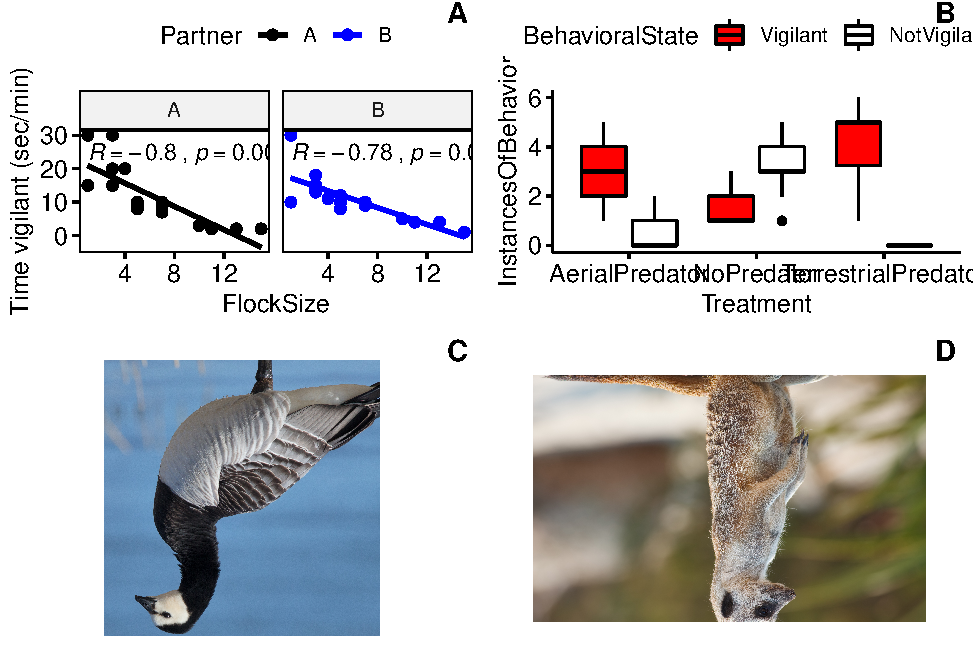
\includegraphics{behaviouR-R-package-tutorials_files/figure-latex/unnamed-chunk-87-1.pdf}

Then we extract the features, which in this case are the MFCCs.

\begin{Shaded}
\begin{Highlighting}[]
\NormalTok{MySoundscapeFeatureDataframe <-}\StringTok{ }
\StringTok{  }\KeywordTok{MFCCFunctionSite}\NormalTok{(}\DataTypeTok{input.dir =} \StringTok{"MySoundscapeRecordings"}\NormalTok{,}\DataTypeTok{min.freq =} \DecValTok{200}\NormalTok{,}\DataTypeTok{max.freq=}\DecValTok{10000}\NormalTok{)}
\end{Highlighting}
\end{Shaded}

Check the resulting structure of the dataframe to make sure it looks OK.

\begin{Shaded}
\begin{Highlighting}[]
\KeywordTok{dim}\NormalTok{(MySoundscapeFeatureDataframe)}
\end{Highlighting}
\end{Shaded}

Now we visualize our results

\begin{Shaded}
\begin{Highlighting}[]
\NormalTok{pca_res <-}\StringTok{ }\KeywordTok{prcomp}\NormalTok{(MySoundscapeFeatureDataframe[,}\OperatorTok{-}\KeywordTok{c}\NormalTok{(}\DecValTok{1}\NormalTok{)], }\DataTypeTok{scale. =} \OtherTok{TRUE}\NormalTok{)}
\NormalTok{ggplot2}\OperatorTok{::}\KeywordTok{autoplot}\NormalTok{(pca_res, }\DataTypeTok{data =}\NormalTok{ MySoundscapeFeatureDataframe, }
         \DataTypeTok{colour =} \StringTok{'Class'}\NormalTok{)}
\end{Highlighting}
\end{Shaded}

\includegraphics{behaviouR-R-package-tutorials_files/figure-latex/unnamed-chunk-90-1.pdf}

\emph{Question 4}. Do you see evidence of clustering in either your focal recordings or soundscape recordings?

\hypertarget{lab-4.-vigilance-behavior}{%
\chapter{Lab 4. Vigilance behavior}\label{lab-4.-vigilance-behavior}}

\begin{center}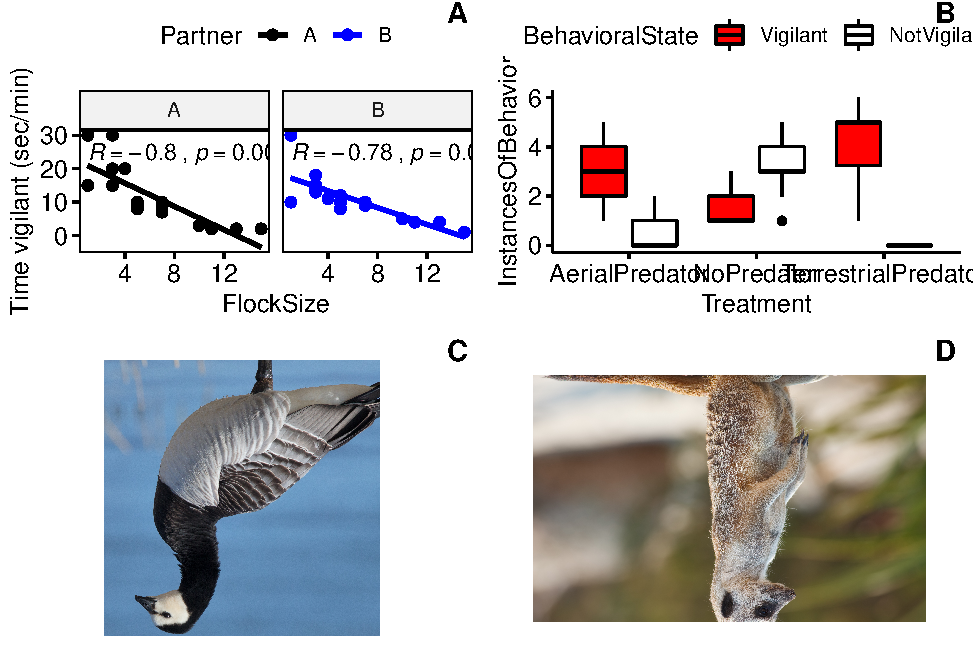
\includegraphics{behaviouR-R-package-tutorials_files/figure-latex/unnamed-chunk-91-1} \end{center}

\emph{Background}\\
In this lab we will continue our work investigating vigilance behaviors in geese and meerkats.

\emph{Goals of the exercises}\\
The main goal(s) of today's lab are to:\\
1) Use the data on goose vigilance behavior to investigate the relationship between group size and vigilance behaviors.\\
2) Analyze the data collected during the meerkat lab to test for differences in vigilant behavior across predator treatment groups.\\
3) Continue to become familar with the way scientists analyze and interpret data.

\emph{Getting started}\\
First we need to load the relevant packages for our data analysis. Packages contain all the functions that are needed for data analysis.
First we load the required libraries

\begin{Shaded}
\begin{Highlighting}[]
\KeywordTok{library}\NormalTok{(behaviouR)}
\end{Highlighting}
\end{Shaded}

\hypertarget{part-1-barnacle-goose-vigilance}{%
\section{Part 1: Barnacle goose vigilance}\label{part-1-barnacle-goose-vigilance}}

We load in our goose data

\begin{Shaded}
\begin{Highlighting}[]
\NormalTok{BarnacleGooseData <-}\StringTok{ }\KeywordTok{read.csv}\NormalTok{(}\StringTok{'BarnacleGooseData.csv'}\NormalTok{)}
\end{Highlighting}
\end{Shaded}

\hypertarget{part-1a-surveillance-behavior}{%
\subsection{Part 1a: Surveillance behavior}\label{part-1a-surveillance-behavior}}

First, we will calculate the surveillance rate (or the number of heads up per minute). Let's start by looking at the total number of `head up' behaviors in our ethogram. To investigate this relationship we will create a scatterplot.

\begin{Shaded}
\begin{Highlighting}[]
\CommentTok{# Scatterplot of total number of 'head up' in our data}
\KeywordTok{ggscatter}\NormalTok{(}\DataTypeTok{data=}\NormalTok{BarnacleGooseData,}
          \DataTypeTok{x=}\StringTok{'FlockSize'}\NormalTok{,}\DataTypeTok{y=}\StringTok{'TotalHeadsUp'}\NormalTok{)}\OperatorTok{+}\KeywordTok{ylab}\NormalTok{(}\StringTok{'Surveillance rate'}\NormalTok{)}
\end{Highlighting}
\end{Shaded}

\includegraphics{behaviouR-R-package-tutorials_files/figure-latex/unnamed-chunk-95-1.pdf}

Now let's add a trend line to see if there is a relationship between flock size and the total number of `head up' behaviors

\begin{Shaded}
\begin{Highlighting}[]
\NormalTok{knitr}\OperatorTok{::}\NormalTok{opts_chunk}\OperatorTok{$}\KeywordTok{set}\NormalTok{(}\DataTypeTok{fig.height =} \DecValTok{5}\NormalTok{, }\DataTypeTok{fig.width =} \DecValTok{5}\NormalTok{)}
\CommentTok{# Scatterplot of total number of 'head up' in our data with a trend line.}

\KeywordTok{ggscatter}\NormalTok{(}\DataTypeTok{data=}\NormalTok{BarnacleGooseData,}
          \DataTypeTok{x=}\StringTok{'FlockSize'}\NormalTok{,}\DataTypeTok{y=}\StringTok{'TotalHeadsUp'}\NormalTok{,}\DataTypeTok{add=}\StringTok{'reg.line'}\NormalTok{)}\OperatorTok{+}\KeywordTok{ylab}\NormalTok{(}\StringTok{'Surveillance rate'}\NormalTok{)}
\end{Highlighting}
\end{Shaded}

\includegraphics{behaviouR-R-package-tutorials_files/figure-latex/unnamed-chunk-96-1.pdf}

Let's see if there were any differences between you and your partner. We will also add the command `cor.coef = T' which will give us the correlation coefficient (R) along with an associated p-value.

\begin{Shaded}
\begin{Highlighting}[]
\CommentTok{# }\AlertTok{NOTE}\CommentTok{: The data here are simulated so your plots should look different}
\KeywordTok{ggscatter}\NormalTok{(}\DataTypeTok{data=}\NormalTok{BarnacleGooseData,}
          \DataTypeTok{x=}\StringTok{'FlockSize'}\NormalTok{,}\DataTypeTok{y=}\StringTok{'TotalHeadsUp'}\NormalTok{,}\DataTypeTok{add=}\StringTok{'reg.line'}\NormalTok{, }\DataTypeTok{facet.by =} \StringTok{'Partner'}\NormalTok{,}
          \DataTypeTok{cor.coef =}\NormalTok{ T)}\OperatorTok{+}\KeywordTok{ylab}\NormalTok{(}\StringTok{'Surveillance rate'}\NormalTok{)}
\end{Highlighting}
\end{Shaded}

\includegraphics{behaviouR-R-package-tutorials_files/figure-latex/unnamed-chunk-97-1.pdf}

Let's plot you and your partner's data in different colors.

\begin{Shaded}
\begin{Highlighting}[]
\KeywordTok{ggscatter}\NormalTok{(}\DataTypeTok{data=}\NormalTok{BarnacleGooseData,}
          \DataTypeTok{x=}\StringTok{'FlockSize'}\NormalTok{,}\DataTypeTok{y=}\StringTok{'TotalHeadsUp'}\NormalTok{,}\DataTypeTok{add=}\StringTok{'reg.line'}\NormalTok{, }\DataTypeTok{facet.by =} \StringTok{'Partner'}\NormalTok{,}
          \DataTypeTok{color =} \StringTok{'Partner'}\NormalTok{, }\DataTypeTok{palette =}\KeywordTok{c}\NormalTok{(}\StringTok{'black'}\NormalTok{,}\StringTok{'blue'}\NormalTok{),}
          \DataTypeTok{cor.coef =}\NormalTok{ T)}\OperatorTok{+}\KeywordTok{ylab}\NormalTok{(}\StringTok{'Surveillance rate'}\NormalTok{)}
\end{Highlighting}
\end{Shaded}

\includegraphics{behaviouR-R-package-tutorials_files/figure-latex/unnamed-chunk-98-1.pdf}

\textbf{Question 1}: Were there any major differences between you and your partner in terms of the observed relationship between flock size and surveillance rate?

Now we will do model selection using Akaike information criterion (AIC). First we create a null model and then we create a model with flock size as a predictor of total number of heads up.In the model code we specify that we are using a Poisson distribution, as we are dealing with count data instead of a continuous variable.

\begin{Shaded}
\begin{Highlighting}[]
\CommentTok{# This is our null model}
\NormalTok{SurveillanceNullModel <-}\StringTok{ }\KeywordTok{glm}\NormalTok{(TotalHeadsUp }\OperatorTok{~}\StringTok{ }\NormalTok{(}\DecValTok{1}\OperatorTok{/}\NormalTok{Partner),}\DataTypeTok{family=}\NormalTok{poisson , }\DataTypeTok{data=}\NormalTok{BarnacleGooseData)}

\CommentTok{# This is our model with flock size as a predictor of total number of heads up}
\NormalTok{SurveillanceModel <-}\StringTok{ }\KeywordTok{glm}\NormalTok{(TotalHeadsUp }\OperatorTok{~}\StringTok{ }\NormalTok{FlockSize }\OperatorTok{+}\StringTok{ }\NormalTok{(}\DecValTok{1}\OperatorTok{/}\NormalTok{Partner) ,}\DataTypeTok{family=}\NormalTok{poisson, }\DataTypeTok{data=}\NormalTok{BarnacleGooseData)}

\CommentTok{# Then we compare the models using AIC}
\NormalTok{bbmle}\OperatorTok{::}\KeywordTok{AICtab}\NormalTok{(SurveillanceNullModel,SurveillanceModel)}
\end{Highlighting}
\end{Shaded}

\begin{verbatim}
##                       dAIC df
## SurveillanceNullModel 0.0  1 
## SurveillanceModel     1.6  2
\end{verbatim}

\textbf{Question 2}: If the null model is ranked higher than the model with flock size as a predictor, how do would we interpret this finding? What if the model with flock size as a predictor was ranked higher? What were your results?

\hypertarget{part-1b-time-vigilant-secmin}{%
\subsection{Part 1b: Time vigilant (sec/min)}\label{part-1b-time-vigilant-secmin}}

Now we will look at the relationship between the duration (calculated as seconds per minute) that the geese were vigilant as a function of flock size.

\begin{Shaded}
\begin{Highlighting}[]
\CommentTok{# Scatterplot of time vigilant (sec/min) as a function of group size}
\KeywordTok{ggscatter}\NormalTok{(}\DataTypeTok{data=}\NormalTok{BarnacleGooseData,}
          \DataTypeTok{x=}\StringTok{'FlockSize'}\NormalTok{,}\DataTypeTok{y=}\StringTok{'TimeSecHeadUp'}\NormalTok{)}\OperatorTok{+}\KeywordTok{ylab}\NormalTok{(}\StringTok{'time vigilant (sec/min)'}\NormalTok{)}
\end{Highlighting}
\end{Shaded}

\includegraphics{behaviouR-R-package-tutorials_files/figure-latex/unnamed-chunk-100-1.pdf}

Now let's add a trend line to see if there is a relationship between flock size and the duration of vigilance.

\begin{Shaded}
\begin{Highlighting}[]
\CommentTok{# Scatterplot of duration of vigilance behavior in our data with a trend line.}

\KeywordTok{ggscatter}\NormalTok{(}\DataTypeTok{data=}\NormalTok{BarnacleGooseData,}\DataTypeTok{x=}\StringTok{'FlockSize'}\NormalTok{,}\DataTypeTok{y=}\StringTok{'TimeSecHeadUp'}\NormalTok{,}\DataTypeTok{add=}\StringTok{'reg.line'}\NormalTok{)}\OperatorTok{+}
\StringTok{  }\KeywordTok{ylab}\NormalTok{(}\StringTok{'time vigilant (sec/min)'}\NormalTok{)}
\end{Highlighting}
\end{Shaded}

\includegraphics{behaviouR-R-package-tutorials_files/figure-latex/unnamed-chunk-101-1.pdf}

Let's see if there were any differences between you and your partner. We will also add the command `cor.coef = T' which will give us the correlation coefficient (R) along with an associated p-value.

\begin{Shaded}
\begin{Highlighting}[]
\CommentTok{# }\AlertTok{NOTE}\CommentTok{: The data here are simulated so your plots should look different}
\KeywordTok{ggscatter}\NormalTok{(}\DataTypeTok{data=}\NormalTok{BarnacleGooseData,}\DataTypeTok{x=}\StringTok{'FlockSize'}\NormalTok{,}\DataTypeTok{y=}\StringTok{'TimeSecHeadUp'}\NormalTok{,}\DataTypeTok{add=}\StringTok{'reg.line'}\NormalTok{,}
          \DataTypeTok{facet.by =} \StringTok{'Partner'}\NormalTok{,}\DataTypeTok{cor.coef =}\NormalTok{ T)}\OperatorTok{+}
\StringTok{  }\KeywordTok{ylab}\NormalTok{(}\StringTok{'time vigilant (sec/min)'}\NormalTok{)}
\end{Highlighting}
\end{Shaded}

\includegraphics{behaviouR-R-package-tutorials_files/figure-latex/unnamed-chunk-102-1.pdf}

Let's plot you and your partner's data in different colors.

\begin{Shaded}
\begin{Highlighting}[]
\KeywordTok{ggscatter}\NormalTok{(}\DataTypeTok{data=}\NormalTok{BarnacleGooseData,}\DataTypeTok{x=}\StringTok{'FlockSize'}\NormalTok{,}\DataTypeTok{y=}\StringTok{'TimeSecHeadUp'}\NormalTok{,}\DataTypeTok{add=}\StringTok{'reg.line'}\NormalTok{,}
          \DataTypeTok{facet.by =} \StringTok{'Partner'}\NormalTok{, }\DataTypeTok{color=}\StringTok{'Partner'}\NormalTok{, }\DataTypeTok{cor.coef =}\NormalTok{ T,}
          \DataTypeTok{palette =}\KeywordTok{c}\NormalTok{(}\StringTok{'black'}\NormalTok{,}\StringTok{'blue'}\NormalTok{))}\OperatorTok{+}
\StringTok{            }\KeywordTok{ylab}\NormalTok{(}\StringTok{'time vigilant (sec/min)'}\NormalTok{)}
\end{Highlighting}
\end{Shaded}

\includegraphics{behaviouR-R-package-tutorials_files/figure-latex/unnamed-chunk-103-1.pdf}

As before we will create a null model and then a model with flock size as a predictor and compare them using AIC. We will not use a Poisson distribution here because our outcome variable is continuous.

\begin{Shaded}
\begin{Highlighting}[]
\CommentTok{# This is our null model}
\NormalTok{VigilanceNullModel <-}\StringTok{ }\NormalTok{lme4}\OperatorTok{::}\KeywordTok{lmer}\NormalTok{(TimeSecHeadUp }\OperatorTok{~}\StringTok{ }\NormalTok{(}\DecValTok{1}\OperatorTok{|}\NormalTok{Partner), }\DataTypeTok{data=}\NormalTok{BarnacleGooseData)}

\CommentTok{# This is our model with flock size as a predictor duration of vigilance}
\NormalTok{VigilanceModel <-}\StringTok{ }\NormalTok{lme4}\OperatorTok{::}\KeywordTok{lmer}\NormalTok{(TimeSecHeadUp }\OperatorTok{~}\StringTok{ }\NormalTok{FlockSize }\OperatorTok{+}\StringTok{ }\NormalTok{(}\DecValTok{1}\OperatorTok{|}\NormalTok{Partner) ,}\DataTypeTok{data=}\NormalTok{BarnacleGooseData)}

\CommentTok{# Now we compare the models using AIC}
\NormalTok{bbmle}\OperatorTok{::}\KeywordTok{AICtab}\NormalTok{(VigilanceNullModel,VigilanceModel)}
\end{Highlighting}
\end{Shaded}

\begin{verbatim}
##                    dAIC df
## VigilanceModel      0.0 4 
## VigilanceNullModel 28.1 3
\end{verbatim}

\#\textbf{Question 3.} How do you interpret the results of your model selection? Was there a relationship between flock size and duration of vigilance behavior?

\hypertarget{part-2-meerkat-data-revisted}{%
\section{Part 2: Meerkat data revisted}\label{part-2-meerkat-data-revisted}}

Please upload your meerkat scan data to this project and delete the existing datasheet.

\begin{Shaded}
\begin{Highlighting}[]
\NormalTok{MeerkatScanData <-}\StringTok{ }\KeywordTok{read.csv}\NormalTok{(}\StringTok{'MeerkatScanData.csv'}\NormalTok{)}
\end{Highlighting}
\end{Shaded}

As before we will turn our NA values to zero

\begin{Shaded}
\begin{Highlighting}[]
\NormalTok{MeerkatScanData[}\KeywordTok{is.na}\NormalTok{(MeerkatScanData)] <-}\StringTok{ '0'}
\end{Highlighting}
\end{Shaded}

We will remove the time and out of sight columns as we do not need them

\begin{Shaded}
\begin{Highlighting}[]
\NormalTok{MeerkatScanData <-}\StringTok{ }\NormalTok{dplyr}\OperatorTok{::}\KeywordTok{select}\NormalTok{(MeerkatScanData,}\OperatorTok{-}\KeywordTok{c}\NormalTok{(Time,OutOfSight))}
\end{Highlighting}
\end{Shaded}

We need to reformat our data so that we can plot it

\begin{Shaded}
\begin{Highlighting}[]
\NormalTok{MeerkatScanDataSummaryLong <-}\StringTok{ }\NormalTok{reshape2}\OperatorTok{::}\KeywordTok{melt}\NormalTok{(MeerkatScanData, }\DataTypeTok{id.vars=}\KeywordTok{c}\NormalTok{(}\StringTok{"Treatment"}\NormalTok{, }\StringTok{"Partner"}\NormalTok{))}
\end{Highlighting}
\end{Shaded}

Here we add more informative column names

\begin{Shaded}
\begin{Highlighting}[]
\KeywordTok{colnames}\NormalTok{(MeerkatScanDataSummaryLong) <-}\StringTok{ }\KeywordTok{c}\NormalTok{(}\StringTok{'Treatment'}\NormalTok{,}\StringTok{'Partner'}\NormalTok{,}
                                          \StringTok{'BehavioralState'}\NormalTok{,}\StringTok{'InstancesOfBehavior'}\NormalTok{)}
\end{Highlighting}
\end{Shaded}

We need to tell R that our outcome variable is not categorical but numeric

\begin{Shaded}
\begin{Highlighting}[]
\NormalTok{MeerkatScanDataSummaryLong}\OperatorTok{$}\NormalTok{InstancesOfBehavior <-}\StringTok{ }
\StringTok{  }\KeywordTok{as.numeric}\NormalTok{(MeerkatScanDataSummaryLong}\OperatorTok{$}\NormalTok{InstancesOfBehavior)}
\end{Highlighting}
\end{Shaded}

Now we plot our data.

\begin{Shaded}
\begin{Highlighting}[]
\KeywordTok{ggboxplot}\NormalTok{(MeerkatScanDataSummaryLong,}\DataTypeTok{x=}\StringTok{'Treatment'}\NormalTok{,}
          \DataTypeTok{y=}\StringTok{'InstancesOfBehavior'}\NormalTok{, }\DataTypeTok{fill =} \StringTok{'BehavioralState'}\NormalTok{)}\OperatorTok{+}\KeywordTok{scale_fill_manual}\NormalTok{(}\DataTypeTok{values =} \KeywordTok{c}\NormalTok{(}\StringTok{'red'}\NormalTok{,}\StringTok{'white'}\NormalTok{,}\StringTok{'black'}\NormalTok{))}
\end{Highlighting}
\end{Shaded}

\includegraphics{behaviouR-R-package-tutorials_files/figure-latex/unnamed-chunk-112-1.pdf}

\textbf{Question 4.} Based on your inspection of the boxplots, are there any major differences between treatment groups?

Now we will test to see if there were differences in vigilance behaviors across treatments.

\begin{Shaded}
\begin{Highlighting}[]
\CommentTok{# First we subset our data so that it only includes the vigilant category}
\NormalTok{MeerkatScanDataVigilantOnly <-}\StringTok{ }\KeywordTok{subset}\NormalTok{(MeerkatScanDataSummaryLong,}
\NormalTok{                                      BehavioralState}\OperatorTok{==}\StringTok{'Vigilant'}\NormalTok{ )}

\CommentTok{# R can be picky about the format of data, so we use this command to tell R that treatment group is a factor}
\NormalTok{MeerkatScanDataVigilantOnly}\OperatorTok{$}\NormalTok{Treatment <-}\StringTok{ }
\StringTok{  }\KeywordTok{as.factor}\NormalTok{(MeerkatScanDataVigilantOnly}\OperatorTok{$}\NormalTok{Treatment)}

\CommentTok{# Here we are reordering the levels of the factors. For our model selection we are interested in whether we see differences from the control (no predator) and the predator treatments, so here we are setting the no predator group as our reference group.}

\NormalTok{MeerkatScanDataVigilantOnly}\OperatorTok{$}\NormalTok{Treatment <-}\StringTok{ }
\StringTok{  }\KeywordTok{factor}\NormalTok{(MeerkatScanDataVigilantOnly}\OperatorTok{$}\NormalTok{Treatment, }\DataTypeTok{levels =} \KeywordTok{c}\NormalTok{(}\StringTok{"NoPredator"}\NormalTok{, }\StringTok{"AerialPredator"}\NormalTok{, }
                                                           \StringTok{"TerrestrialPredator"}\NormalTok{))}
\end{Highlighting}
\end{Shaded}

Now as before we will do model selection. Note that because our outcome variable (instances of behavior) is in the form of count data we use a poisson distribution.

\begin{Shaded}
\begin{Highlighting}[]
\CommentTok{# This is the null model.}
\NormalTok{MeerkatVigilanceNullModel <-}\StringTok{ }\KeywordTok{glm}\NormalTok{(InstancesOfBehavior }\OperatorTok{~}\StringTok{ }\DecValTok{1}\NormalTok{, }\DataTypeTok{family=}\NormalTok{poisson, }\DataTypeTok{data=}\NormalTok{MeerkatScanDataVigilantOnly)}

\CommentTok{# This is the model with treatment as a predictor of instances of vigilant behavior}
\NormalTok{MeerkatVigilanceModel <-}\StringTok{ }\KeywordTok{glm}\NormalTok{(InstancesOfBehavior }\OperatorTok{~}\StringTok{ }\NormalTok{Treatment, }\DataTypeTok{family=}\NormalTok{poisson,}\DataTypeTok{data=}\NormalTok{MeerkatScanDataVigilantOnly)}
\end{Highlighting}
\end{Shaded}

Now we compare the models using AIC

\begin{Shaded}
\begin{Highlighting}[]
\NormalTok{bbmle}\OperatorTok{::}\KeywordTok{AICtab}\NormalTok{(MeerkatVigilanceNullModel,MeerkatVigilanceModel)}
\end{Highlighting}
\end{Shaded}

\begin{verbatim}
##                           dAIC df
## MeerkatVigilanceModel      0.0 3 
## MeerkatVigilanceNullModel 59.2 1
\end{verbatim}

Here we will use the summary function to look at the estimates. There is a lot of information here but we want to focus on the `Estimate'. In particular we are interested in the estimates for `TreatmentAerialPredator' and `TreatmentTerrestrialPredator'. The estimate is showing the effect that these variables have on our outcome (instances of behavior), relative to our control (no predator).Therefore positive estimates indicate that there were more vigilance behaviors in aerial and terrestrial predator treatments.

\begin{Shaded}
\begin{Highlighting}[]
\KeywordTok{summary}\NormalTok{(MeerkatVigilanceModel)}
\end{Highlighting}
\end{Shaded}

\begin{verbatim}
## 
## Call:
## glm(formula = InstancesOfBehavior ~ Treatment, family = poisson, 
##     data = MeerkatScanDataVigilantOnly)
## 
## Deviance Residuals: 
##     Min       1Q   Median       3Q      Max  
## -1.9295  -0.3475  -0.1588   0.3696   1.1825  
## 
## Coefficients:
##                              Estimate Std. Error z value Pr(>|z|)    
## (Intercept)                    0.3285     0.1414   2.323   0.0202 *  
## TreatmentAerialPredator        0.8671     0.1685   5.145 2.68e-07 ***
## TreatmentTerrestrialPredator   1.1362     0.1582   7.182 6.86e-13 ***
## ---
## Signif. codes:  0 '***' 0.001 '**' 0.01 '*' 0.05 '.' 0.1 ' ' 1
## 
## (Dispersion parameter for poisson family taken to be 1)
## 
##     Null deviance: 100.802  on 117  degrees of freedom
## Residual deviance:  37.587  on 115  degrees of freedom
## AIC: 384.39
## 
## Number of Fisher Scoring iterations: 4
\end{verbatim}

A common way to visulize results such as these are coefficient plots. Here we are looking at the effect of `TreatmentAerialPredator' and `TreatmentTerrestrialPredator' relative to our control group. The reference or group is indicated by the vertical dashed line. So, we can interpret that because the coefficients are positive (and the confidence intervals don't overlap zero) that both terrestrial and aerial treatments lead to an increase in vigilant behaviors.

\begin{Shaded}
\begin{Highlighting}[]
\NormalTok{coefplot}\OperatorTok{::}\KeywordTok{coefplot}\NormalTok{(MeerkatVigilanceModel,}\DataTypeTok{intercept=}\NormalTok{F)}
\end{Highlighting}
\end{Shaded}

\includegraphics{behaviouR-R-package-tutorials_files/figure-latex/unnamed-chunk-117-1.pdf}

For reasons that will not go into here, I am not a fan of p-values or null hypothesis significance testing. There is a nice overview if you want to learn more here: \url{https://doi.org/10.1098/rsbl.2019.0174}. But,the model selection approach we used will lead to the same inference as the use of a one-way anova, an approach that you may be more familiar with.

Compute the analysis of variance

\begin{Shaded}
\begin{Highlighting}[]
\NormalTok{MeerkatAOV <-}\StringTok{ }\KeywordTok{aov}\NormalTok{(InstancesOfBehavior }\OperatorTok{~}\StringTok{ }\NormalTok{Treatment, }\DataTypeTok{data =}\NormalTok{ MeerkatScanDataVigilantOnly)}
\end{Highlighting}
\end{Shaded}

Here this will tell us if there are differences between groups. A significant p-value (\textless{} 0.05) indicates there are differences between treatment groups.

\begin{Shaded}
\begin{Highlighting}[]
\KeywordTok{summary}\NormalTok{(MeerkatAOV)}
\end{Highlighting}
\end{Shaded}

\begin{verbatim}
##              Df Sum Sq Mean Sq F value Pr(>F)    
## Treatment     2  176.0   88.02   87.03 <2e-16 ***
## Residuals   115  116.3    1.01                   
## ---
## Signif. codes:  0 '***' 0.001 '**' 0.01 '*' 0.05 '.' 0.1 ' ' 1
\end{verbatim}

Since the ANOVA test is significant, we can compute Tukey Honest Significant Differences test. Again, a significant p-value (\textless{} 0.05) indicates there are differences between treatments.

\begin{Shaded}
\begin{Highlighting}[]
\KeywordTok{TukeyHSD}\NormalTok{(MeerkatAOV)}
\end{Highlighting}
\end{Shaded}

\begin{verbatim}
##   Tukey multiple comparisons of means
##     95% family-wise confidence level
## 
## Fit: aov(formula = InstancesOfBehavior ~ Treatment, data = MeerkatScanDataVigilantOnly)
## 
## $Treatment
##                                        diff       lwr      upr   p adj
## AerialPredator-NoPredator          1.916667 1.3538432 2.479490 0.0e+00
## TerrestrialPredator-NoPredator     2.937198 2.4058425 3.468554 0.0e+00
## TerrestrialPredator-AerialPredator 1.020531 0.4891758 1.551887 3.8e-05
\end{verbatim}

\textbf{Question 5.} Based on your interpretation of the model selection and the coefficient plots were there differences between treatment groups (e.g.~control, terrestrial and aerial predators) in meerkat vigilance behavior?

\hypertarget{lab-5.-estimating-population-density-and-biodiversity}{%
\chapter{Lab 5. Estimating Population Density and Biodiversity}\label{lab-5.-estimating-population-density-and-biodiversity}}

\begin{center}\includegraphics{behaviouR-R-package-tutorials_files/figure-latex/unnamed-chunk-121-1} \end{center}

\emph{Background}\\
In this lab you will become familiar with the ways that scientists estimate population density and biodiversity of terrestrial vertebrates.

\emph{Goals of the exercises}\\
The main goal(s) of today's lab are to:\\
1) Estimate population density of focal vertebrates from the field lab.\\
2) Learn the difference between alpha, beta and gamma diversity.\\
3) Compare population density and biodiversity across your sampling sites.

\emph{Getting started}\\
First we need to load the relevant packages for our data analysis. Packages contain all the functions that are needed for data analysis.

\begin{Shaded}
\begin{Highlighting}[]
\KeywordTok{library}\NormalTok{(behaviouR)}
\end{Highlighting}
\end{Shaded}

Then we read in our data

\begin{Shaded}
\begin{Highlighting}[]
\NormalTok{CensusData <-}\StringTok{ }\KeywordTok{read.csv}\NormalTok{(}\StringTok{'FieldLab5CensusData.csv'}\NormalTok{)}
\end{Highlighting}
\end{Shaded}

\hypertarget{part-1.-population-density-estimation.}{%
\section{Part 1. Population density estimation.}\label{part-1.-population-density-estimation.}}

First let's focus on your data.\\
NOTE: you need to change `A' to the name you used!

\begin{Shaded}
\begin{Highlighting}[]
\NormalTok{MyCensusData <-}\StringTok{ }\KeywordTok{subset}\NormalTok{(CensusData, Partner}\OperatorTok{==}\StringTok{'A'}\NormalTok{)}
\end{Highlighting}
\end{Shaded}

Now we will subset the data to focus on your focal species for density estimation. NOTE: in this example we are subsetting the data so that we only have the squirrels; you will need to change the code to subset based on your focal species!

\begin{Shaded}
\begin{Highlighting}[]
\NormalTok{MyCensusDataFocal <-}\StringTok{ }\KeywordTok{subset}\NormalTok{(MyCensusData, Species}\OperatorTok{==}\StringTok{'squirrel'}\NormalTok{)}
\end{Highlighting}
\end{Shaded}

Here we will determine the width of our sampling area by creating a histogram of perpendicular detection distances. We will identify the point where our detections start to dropoff. We will assume that after this point our ability to detect animals past that distance drops substantially, and including observations past this distance could potentially bias our results.

\begin{Shaded}
\begin{Highlighting}[]
\KeywordTok{hist}\NormalTok{(MyCensusDataFocal}\OperatorTok{$}\NormalTok{PerpendicularDistance,}\DataTypeTok{xlab=}\StringTok{'Perpendicular distance (D)'}\NormalTok{,}
  \DataTypeTok{ylab=}\StringTok{'Number of observations'}\NormalTok{,}\DataTypeTok{main=}\StringTok{''}\NormalTok{)}
\end{Highlighting}
\end{Shaded}

\includegraphics{behaviouR-R-package-tutorials_files/figure-latex/unnamed-chunk-127-1.pdf}

In this example there is a clear break between 15 and 20 meters, so we will only use observations that were within 15 meters.\\
NOTE: Your data will look different than this!

Change the value (in this example 15) to the cutoff point indicated in your data!

\begin{Shaded}
\begin{Highlighting}[]
\NormalTok{CutOffPoint <-}\StringTok{ }\DecValTok{15}
\end{Highlighting}
\end{Shaded}

\begin{Shaded}
\begin{Highlighting}[]
\CommentTok{# Here we subset our data so that it only includes detections that were within 15 meters of the census route}
\NormalTok{MyCensusDataFocalAdjusted <-}\StringTok{ }\KeywordTok{subset}\NormalTok{(MyCensusDataFocal,PerpendicularDistance }\OperatorTok{<}\NormalTok{CutOffPoint )}
\end{Highlighting}
\end{Shaded}

Now we need to subset by each site.\\
NOTE: You will need to change to the site names you used

\begin{Shaded}
\begin{Highlighting}[]
\NormalTok{MyCensusDataFocalSiteA <-}\StringTok{ }\KeywordTok{subset}\NormalTok{(MyCensusDataFocalAdjusted,Site}\OperatorTok{==}\StringTok{'SiteA'}\NormalTok{)}

\NormalTok{MyCensusDataFocalSiteB <-}\StringTok{ }\KeywordTok{subset}\NormalTok{(MyCensusDataFocalAdjusted,Site}\OperatorTok{==}\StringTok{'SiteB'}\NormalTok{)}
\end{Highlighting}
\end{Shaded}

Now we will calculate the population density based on our two surveys. Change the following to indicate the distance (in meters) of your survey for site A. This will be the actual straight-line distance you walked.

\begin{Shaded}
\begin{Highlighting}[]
\NormalTok{SiteACensusDistance <-}\StringTok{ }\DecValTok{500}
\end{Highlighting}
\end{Shaded}

Now we will calculate the area of our census. The sample area (a) is equal to the length of the transect multiplied by twice the width or a= 2wl. We divide by 1000 to convert our answer to square kilometers.

\begin{Shaded}
\begin{Highlighting}[]
\NormalTok{SiteACensusArea <-}\StringTok{ }\DecValTok{2}\OperatorTok{*}\NormalTok{SiteACensusDistance}\OperatorTok{*}\NormalTok{CutOffPoint}\OperatorTok{/}\DecValTok{1000}
\NormalTok{SiteACensusArea}
\end{Highlighting}
\end{Shaded}

\begin{verbatim}
## [1] 15
\end{verbatim}

Now we need to calculate the number of focal animals observed using the following code.

\begin{Shaded}
\begin{Highlighting}[]
\NormalTok{NumberFocalAnimalsSiteA <-}\StringTok{ }\KeywordTok{nrow}\NormalTok{(MyCensusDataFocalSiteA)}
\end{Highlighting}
\end{Shaded}

Then we can calculate the density by dividing the total number of animals we observed by the area we censused.

\begin{Shaded}
\begin{Highlighting}[]
\NormalTok{PopulationDensitySiteA <-NumberFocalAnimalsSiteA}\OperatorTok{/}\NormalTok{SiteACensusArea}
\NormalTok{PopulationDensitySiteA}
\end{Highlighting}
\end{Shaded}

\begin{verbatim}
## [1] 0.4666667
\end{verbatim}

Now we will calculate the population density based on our second survey. Change the following to indicate the distance (in meters) of your survey for site B.This will be the actual straight-line distance you walked.

\begin{Shaded}
\begin{Highlighting}[]
\NormalTok{SiteBCensusDistance <-}\StringTok{ }\DecValTok{500}
\end{Highlighting}
\end{Shaded}

Now we will calculate the area of our census. The sample area (a) is equal to the length of the transect multiplied by twice the width or a= 2wl.We divide by 1000 to convert our answer to square kilometers.

\begin{Shaded}
\begin{Highlighting}[]
\NormalTok{SiteBCensusArea <-}\StringTok{ }\DecValTok{2}\OperatorTok{*}\NormalTok{SiteBCensusDistance}\OperatorTok{*}\NormalTok{CutOffPoint}\OperatorTok{/}\DecValTok{1000}
\NormalTok{SiteBCensusArea}
\end{Highlighting}
\end{Shaded}

\begin{verbatim}
## [1] 15
\end{verbatim}

Now we need to calculate the number of animals using the following code.

\begin{Shaded}
\begin{Highlighting}[]
\NormalTok{NumberFocalAnimalsSiteB <-}\StringTok{ }\KeywordTok{nrow}\NormalTok{(MyCensusDataFocalSiteB)}
\end{Highlighting}
\end{Shaded}

Then we can calculate the density by dividing the total number of animals we observed by the area we censused.

\begin{Shaded}
\begin{Highlighting}[]
\NormalTok{PopulationDensitySiteB <-NumberFocalAnimalsSiteB}\OperatorTok{/}\NormalTok{SiteBCensusArea}
\NormalTok{PopulationDensitySiteB}
\end{Highlighting}
\end{Shaded}

\begin{verbatim}
## [1] 1.133333
\end{verbatim}

Now we can compare population density using the following code. The code below asks if the population density of site A was higher than site B?

\begin{Shaded}
\begin{Highlighting}[]
\NormalTok{PopulationDensitySiteA }\OperatorTok{>}\StringTok{ }\NormalTok{PopulationDensitySiteB}
\end{Highlighting}
\end{Shaded}

\begin{verbatim}
## [1] FALSE
\end{verbatim}

The code below asks if the population density of site B was higher than site A?

\begin{Shaded}
\begin{Highlighting}[]
\NormalTok{PopulationDensitySiteB }\OperatorTok{>}\StringTok{ }\NormalTok{PopulationDensitySiteA}
\end{Highlighting}
\end{Shaded}

\begin{verbatim}
## [1] TRUE
\end{verbatim}

\textbf{Question 1}. What were the population density estimates (reported as number of individuals per square kilometer) for your two sites? Do your results of the population density estimates match your predictions? Why or why not?

\hypertarget{part-2.-comparing-biodiversity.}{%
\section{Part 2. Comparing biodiversity.}\label{part-2.-comparing-biodiversity.}}

\hypertarget{alpha-diversity.}{%
\subsection{Alpha diversity.}\label{alpha-diversity.}}

First, we will estimate the alpha diversity, or the diversity within a particular area or ecosystem. The alpha diversity is simply the number of different species present at each site.

Here we subset by partner and site A (you may need to change these!)

\begin{Shaded}
\begin{Highlighting}[]
\NormalTok{MyCensusDataSiteA <-}\StringTok{ }\KeywordTok{subset}\NormalTok{(MyCensusData,Partner}\OperatorTok{==}\StringTok{'A'} \OperatorTok{&}\StringTok{ }\NormalTok{Site}\OperatorTok{==}\StringTok{'SiteA'}\NormalTok{)}

\CommentTok{# What were the unique species present?}
\KeywordTok{unique}\NormalTok{(MyCensusDataSiteA}\OperatorTok{$}\NormalTok{Species)}
\end{Highlighting}
\end{Shaded}

\begin{verbatim}
## [1] cardinal  blackird1 rabbit    deer      squirrel  crow     
## Levels: blackird1 cardinal crow deer rabbit squirrel
\end{verbatim}

\begin{Shaded}
\begin{Highlighting}[]
\CommentTok{# How many unique species were there?}
\NormalTok{SiteANumberSpecies <-}\StringTok{ }\KeywordTok{length}\NormalTok{(}\KeywordTok{unique}\NormalTok{(MyCensusDataSiteA}\OperatorTok{$}\NormalTok{Species))}
\NormalTok{SiteANumberSpecies}
\end{Highlighting}
\end{Shaded}

\begin{verbatim}
## [1] 6
\end{verbatim}

Here we subset by partner and site B (you may need to change these!)

\begin{Shaded}
\begin{Highlighting}[]
\NormalTok{MyCensusDataSiteB <-}\StringTok{ }\KeywordTok{subset}\NormalTok{(MyCensusData,Partner}\OperatorTok{==}\StringTok{'A'} \OperatorTok{&}\StringTok{ }\NormalTok{Site}\OperatorTok{==}\StringTok{'SiteB'}\NormalTok{)}

\CommentTok{# What were the unique species present?}
\KeywordTok{unique}\NormalTok{(MyCensusDataSiteB}\OperatorTok{$}\NormalTok{Species)}
\end{Highlighting}
\end{Shaded}

\begin{verbatim}
## [1] squirrel  blackird1 rabbit    deer      crow     
## Levels: blackird1 cardinal crow deer rabbit squirrel
\end{verbatim}

\begin{Shaded}
\begin{Highlighting}[]
\CommentTok{# How many unique species were there?}
\NormalTok{SiteBNumberSpecies <-}\StringTok{ }\KeywordTok{length}\NormalTok{(}\KeywordTok{unique}\NormalTok{(MyCensusDataSiteB}\OperatorTok{$}\NormalTok{Species))}
\NormalTok{SiteBNumberSpecies}
\end{Highlighting}
\end{Shaded}

\begin{verbatim}
## [1] 5
\end{verbatim}

\textbf{Question 2}. Which of your sites had higher species richness (i.e.~number of species)?

\hypertarget{beta-diversity.}{%
\subsection{Beta diversity.}\label{beta-diversity.}}

Now we will estimate beta diversity, which estimates changes in species diversity between ecosystems or along environmental gradients.

\begin{Shaded}
\begin{Highlighting}[]
\CommentTok{# This code tells us which species both sites have in common}
\KeywordTok{intersect}\NormalTok{(}\KeywordTok{unique}\NormalTok{(MyCensusDataSiteA}\OperatorTok{$}\NormalTok{Species),}\KeywordTok{unique}\NormalTok{(MyCensusDataSiteB}\OperatorTok{$}\NormalTok{Species))}
\end{Highlighting}
\end{Shaded}

\begin{verbatim}
## [1] "blackird1" "rabbit"    "deer"      "squirrel"  "crow"
\end{verbatim}

\begin{Shaded}
\begin{Highlighting}[]
\CommentTok{# Now we calculate the number of species in common}
\NormalTok{SpeciesInCommonBothSites <-}\StringTok{ }\KeywordTok{length}\NormalTok{(}\KeywordTok{intersect}\NormalTok{(}\KeywordTok{unique}\NormalTok{(MyCensusDataSiteA}\OperatorTok{$}\NormalTok{Species),}\KeywordTok{unique}\NormalTok{(MyCensusDataSiteB}\OperatorTok{$}\NormalTok{Species))}
\NormalTok{)}
\NormalTok{SpeciesInCommonBothSites}
\end{Highlighting}
\end{Shaded}

\begin{verbatim}
## [1] 5
\end{verbatim}

To investigate community similarity we will calculate Sørenson's index; a value of 1 means exactly the same number of species a value of 0 means no overlap.

Beta diversity = 2c / S1 + S2\\
Where c is the number of species the sites have in common, S1 is the number of species at the first site and S2 is the number of species at the second site

\begin{Shaded}
\begin{Highlighting}[]
\DecValTok{2}\OperatorTok{*}\NormalTok{SpeciesInCommonBothSites}\OperatorTok{/}\StringTok{ }\NormalTok{(SiteANumberSpecies}\OperatorTok{+}\NormalTok{SiteBNumberSpecies)}
\end{Highlighting}
\end{Shaded}

\begin{verbatim}
## [1] 0.9090909
\end{verbatim}

\hypertarget{now-we-will-use-your-partners-data-to-estimate-alpha-diversity}{%
\subsection{Now we will use your partner's data to estimate alpha diversity}\label{now-we-will-use-your-partners-data-to-estimate-alpha-diversity}}

\begin{Shaded}
\begin{Highlighting}[]
\NormalTok{MyPartnersCensusDataSiteA <-}\StringTok{ }\KeywordTok{subset}\NormalTok{(CensusData,Partner}\OperatorTok{==}\StringTok{'B'} \OperatorTok{&}\StringTok{ }\NormalTok{Site}\OperatorTok{==}\StringTok{'SiteC'}\NormalTok{)}
\KeywordTok{unique}\NormalTok{(MyPartnersCensusDataSiteA}\OperatorTok{$}\NormalTok{Species)}
\end{Highlighting}
\end{Shaded}

\begin{verbatim}
## [1] squirrel crow    
## Levels: blackird1 cardinal crow deer rabbit squirrel
\end{verbatim}

\begin{Shaded}
\begin{Highlighting}[]
\KeywordTok{length}\NormalTok{(}\KeywordTok{unique}\NormalTok{(MyPartnersCensusDataSiteA}\OperatorTok{$}\NormalTok{Species))}
\end{Highlighting}
\end{Shaded}

\begin{verbatim}
## [1] 2
\end{verbatim}

\begin{Shaded}
\begin{Highlighting}[]
\NormalTok{SiteANumberSpecies <-}\StringTok{ }\KeywordTok{length}\NormalTok{(}\KeywordTok{unique}\NormalTok{(MyPartnersCensusDataSiteA}\OperatorTok{$}\NormalTok{Species))}
\NormalTok{SiteANumberSpecies}
\end{Highlighting}
\end{Shaded}

\begin{verbatim}
## [1] 2
\end{verbatim}

\begin{Shaded}
\begin{Highlighting}[]
\NormalTok{MyPartnersCensusDataSiteB <-}\StringTok{ }\KeywordTok{subset}\NormalTok{(CensusData,Partner}\OperatorTok{==}\StringTok{'B'} \OperatorTok{&}\StringTok{ }\NormalTok{Site}\OperatorTok{==}\StringTok{'SiteD'}\NormalTok{)}
\KeywordTok{unique}\NormalTok{(MyPartnersCensusDataSiteB}\OperatorTok{$}\NormalTok{Species)}
\end{Highlighting}
\end{Shaded}

\begin{verbatim}
## [1] squirrel
## Levels: blackird1 cardinal crow deer rabbit squirrel
\end{verbatim}

\begin{Shaded}
\begin{Highlighting}[]
\KeywordTok{length}\NormalTok{(}\KeywordTok{unique}\NormalTok{(MyPartnersCensusDataSiteB}\OperatorTok{$}\NormalTok{Species))}
\end{Highlighting}
\end{Shaded}

\begin{verbatim}
## [1] 1
\end{verbatim}

\begin{Shaded}
\begin{Highlighting}[]
\NormalTok{SiteBNumberSpecies <-}\StringTok{ }\KeywordTok{length}\NormalTok{(}\KeywordTok{unique}\NormalTok{(MyPartnersCensusDataSiteB}\OperatorTok{$}\NormalTok{Species))}
\NormalTok{SiteBNumberSpecies}
\end{Highlighting}
\end{Shaded}

\begin{verbatim}
## [1] 1
\end{verbatim}

\textbf{Question 3}. How did the alpha diversity of each of your sites compare with that of your partner?

\hypertarget{gamma-diversity}{%
\subsection{Gamma diversity}\label{gamma-diversity}}

Gamma diversity is the total number of species over a large area or region; there are many different ways that this can be measured. The way we will do it is a bit of an oversimplification by simply comparing the number of species seen during the census at both locations.

First we subset by the first partner

\begin{Shaded}
\begin{Highlighting}[]
\NormalTok{MyCensusData <-}\StringTok{ }\KeywordTok{subset}\NormalTok{(CensusData, Partner}\OperatorTok{==}\StringTok{'A'}\NormalTok{)}
\KeywordTok{unique}\NormalTok{(MyCensusData}\OperatorTok{$}\NormalTok{Species)}
\end{Highlighting}
\end{Shaded}

\begin{verbatim}
## [1] cardinal  blackird1 rabbit    deer      squirrel  crow     
## Levels: blackird1 cardinal crow deer rabbit squirrel
\end{verbatim}

Then we plot the results

\begin{Shaded}
\begin{Highlighting}[]
\KeywordTok{gghistogram}\NormalTok{(}\DataTypeTok{data=}\NormalTok{MyCensusData, }\DataTypeTok{x=}\StringTok{'Species'}\NormalTok{,}\DataTypeTok{stat=}\StringTok{"count"}\NormalTok{)}
\end{Highlighting}
\end{Shaded}

\includegraphics{behaviouR-R-package-tutorials_files/figure-latex/unnamed-chunk-147-1.pdf}

Now we subset by the second partner

\begin{Shaded}
\begin{Highlighting}[]
\NormalTok{MyPartnersCensusData <-}\StringTok{ }\KeywordTok{subset}\NormalTok{(CensusData, Partner}\OperatorTok{==}\StringTok{'B'}\NormalTok{)}
\KeywordTok{unique}\NormalTok{(MyPartnersCensusData}\OperatorTok{$}\NormalTok{Species)}
\end{Highlighting}
\end{Shaded}

\begin{verbatim}
## [1] squirrel crow    
## Levels: blackird1 cardinal crow deer rabbit squirrel
\end{verbatim}

Then we plot the results

\begin{Shaded}
\begin{Highlighting}[]
\KeywordTok{gghistogram}\NormalTok{(}\DataTypeTok{data=}\NormalTok{MyPartnersCensusData, }\DataTypeTok{x=}\StringTok{'Species'}\NormalTok{,}\DataTypeTok{stat=}\StringTok{"count"}\NormalTok{)}
\end{Highlighting}
\end{Shaded}

\includegraphics{behaviouR-R-package-tutorials_files/figure-latex/unnamed-chunk-149-1.pdf}

Now we can plot all the data together, separated by partner

\begin{Shaded}
\begin{Highlighting}[]
\KeywordTok{gghistogram}\NormalTok{(}\DataTypeTok{data=}\NormalTok{CensusData, }\DataTypeTok{x=}\StringTok{'Species'}\NormalTok{,}\DataTypeTok{stat=}\StringTok{"count"}\NormalTok{,}
            \DataTypeTok{facet.by =} \StringTok{'Partner'}\NormalTok{,}\DataTypeTok{x.text.angle =}\DecValTok{90}\NormalTok{,}
            \DataTypeTok{fill=}\StringTok{'Partner'}\NormalTok{)}\OperatorTok{+}\KeywordTok{xlab}\NormalTok{(}\StringTok{'Species'}\NormalTok{)}\OperatorTok{+}\KeywordTok{ylab}\NormalTok{(}\StringTok{'Number of individuals'}\NormalTok{)}
\end{Highlighting}
\end{Shaded}

\includegraphics{behaviouR-R-package-tutorials_files/figure-latex/unnamed-chunk-150-1.pdf}

\textbf{Question 4}. How did the gamma diversity of your site compare with that of your partners?

\hypertarget{part-3.-biodiversity-indices-in-the-real-world.}{%
\section{Part 3. Biodiversity indices in the real world.}\label{part-3.-biodiversity-indices-in-the-real-world.}}

There are special packages in R that can measure different diversity indices, as biodiversity indices are tools many ecologists use. The package we will use is called `vegan'.

\begin{Shaded}
\begin{Highlighting}[]
\KeywordTok{library}\NormalTok{(vegan)}
\end{Highlighting}
\end{Shaded}

First we need to convert our data into a table that can be used to calculate the indices.

\begin{Shaded}
\begin{Highlighting}[]
\NormalTok{BiodiversityTable <-}\StringTok{ }\KeywordTok{table}\NormalTok{(CensusData}\OperatorTok{$}\NormalTok{Site,CensusData}\OperatorTok{$}\NormalTok{Species)}
\end{Highlighting}
\end{Shaded}

Simpson's Index (D) measures the probability that two individuals randomly selected from a sample will belong to the same species (or some category other than species). With this index, 1 represents infinite diversity and 0 means no diversity.

\begin{Shaded}
\begin{Highlighting}[]
\NormalTok{H <-}\StringTok{ }\KeywordTok{diversity}\NormalTok{(BiodiversityTable,}\DataTypeTok{index=}\StringTok{"simpson"}\NormalTok{)}
\NormalTok{H}
\end{Highlighting}
\end{Shaded}

\begin{verbatim}
##     SiteA     SiteB     SiteC     SiteD 
## 0.7962963 0.6728395 0.4444444 0.0000000
\end{verbatim}

Species evenness refers to how close in numbers each species is in an environment. We can calculate evenness using the following code. The value is constrained between 0 and 1, with communities that have a more even representation of species having values closer to 1.

\begin{Shaded}
\begin{Highlighting}[]
\NormalTok{J <-}\StringTok{ }\NormalTok{H}\OperatorTok{/}\KeywordTok{log}\NormalTok{(}\KeywordTok{specnumber}\NormalTok{(BiodiversityTable))}
\NormalTok{J}
\end{Highlighting}
\end{Shaded}

\begin{verbatim}
##     SiteA     SiteB     SiteC     SiteD 
## 0.4444214 0.4180587 0.6411978       NaN
\end{verbatim}

\textbf{Question 5}. Which of the four sites you analyzed was most diverse? Which was the most even? Why is it important to consider diversity and evenness when studying biodiversity?

\hypertarget{lab-6.-analyzing-camera-trap-data.}{%
\chapter{Lab 6. Analyzing camera trap data.}\label{lab-6.-analyzing-camera-trap-data.}}

\begin{center}\includegraphics[width=0.8\linewidth]{behaviouR-R-package-tutorials_files/figure-latex/unnamed-chunk-155-1} \end{center}

\emph{Background}\\
In this lab we will use actual camera trap data collected in Serengeti National Park to investigate temporal niche partitioning. The camera trap data that we will use for this field lab comes from the `Snapshot Serengeti' project (\url{http://lila.science/datasets/snapshot-serengeti}). The scientists set out out 225 cameras within a 1,125 km2 area. The cameras have been deployed continuously since 2010, and the researchers recruited citizen scientists to help with classifying images (\url{https://www.zooniverse.org/projects/zooniverse/snapshot-serengeti}).

\emph{Goals of the exercises}\\
The main goal(s) of today's lab are to:\\
1) Understand the types of behavioral data that scientists can collect from camera trap photos.\\
2) Become familiar with one of the ways scientists can compare differences in activity patterns.\\
3) Think about interspecific interactions of predator-prey and potential competitors in the Serengeti.

\emph{Getting started}\\
First we need to load the relevant packages for our data analysis. Packages contain all the functions that are needed for data analysis.

\begin{Shaded}
\begin{Highlighting}[]
\KeywordTok{library}\NormalTok{(behaviouR)}
\end{Highlighting}
\end{Shaded}

\hypertarget{part-1-collect-serengeti-camera-trap-data}{%
\section{Part 1: Collect Serengeti camera trap data}\label{part-1-collect-serengeti-camera-trap-data}}

The original dataset includes over 2.65M sequences of camera trap images (totaling 7.1M images) from ten field seasons. As you can imagine that is a lot of data! For this lab we will focus on a subset of the data collected over the course of a few seasons.

We will be taking random subsets of the camera trap photos (the current default is 5 per season which you should change for your actual study), and we use `set.seed' to make sure that our results are reproducible.

\begin{Shaded}
\begin{Highlighting}[]
\KeywordTok{set.seed}\NormalTok{(}\DecValTok{2210}\NormalTok{)}
\end{Highlighting}
\end{Shaded}

We can use the following code to query the database by season to see which photos are available. The available seasons are 1-4, 6-8,10,11. This function will return a table with all of the available camera trap photos for a particular season. With camera trap data often times photos will be taken in a sequence (e.g.~if the animal is moving in front of the camera for a long time). The values in the table below include all photos in a sequence, but the code we use to download the photos only takes the first photo in a sequence. Therefore the sample sizes indicated in this table and the actual sample size may be different.

\begin{Shaded}
\begin{Highlighting}[]
\KeywordTok{CameraTrapAnnotations}\NormalTok{(}\DataTypeTok{season =} \DecValTok{1}\NormalTok{)}
\end{Highlighting}
\end{Shaded}

\begin{verbatim}
## 
##        aardvark        aardwolf          baboon     batearedfox         buffalo 
##             143              88             348             315            1455 
##        bushbuck         caracal         cheetah           civet          dikdik 
##              36              57             575              27             728 
##           eland        elephant   gazellegrants gazellethomsons           genet 
##             113            1687            4967           29705              28 
##         giraffe      guineafowl            hare      hartebeest    hippopotamus 
##            1923            3217             327            2139             340 
##     honeybadger    hyenaspotted    hyenastriped          impala          jackal 
##              42            2752             112             691             304 
##     koribustard         leopard      lionfemale        lionmale        mongoose 
##             591              38            1519             665             290 
##    monkeyvervet         ostrich       otherbird       porcupine        reedbuck 
##              64             211            2322             114             946 
##        reptiles      rhinoceros         rodents   secretarybird          serval 
##             357               6             129             198             174 
##            topi         warthog       waterbuck         wildcat      wildebeest 
##             428            2685              25              48             689 
##           zebra         zorilla 
##            5592               9
\end{verbatim}

For this lab you are going to choose two animals from the camera trap dataset. It could be a pair of animals that are predator and prey or two potential competitors. Once you decide on the two animals you want to compare you will make some predictions about how you think they will differ in their activity patterns.

Now we will use another function to download the camera trap photos and save them locally to our computer. You can change the season by changing the values for season (remember the available seasons are 1-4, 6-8,10,11). You can change the focal animal by changing the `AnimalID'; make sure that the spelling and case is exactly the same as in the table above. You can change the number of photos per season that you download (the default is 5). When `create.dir' is true this will create a folder in your current working directory. For this example the folder is called `CameraTrapPhotoszebra'. If create.dir=`FALSE' all the photos will be downloaded directly to your working directory. To find the directory type `getwd()' into your R console.

\begin{Shaded}
\begin{Highlighting}[]
\NormalTok{CombinedAnimalDF <-}\StringTok{ }\KeywordTok{CameraTrapDataAccess}\NormalTok{(}\DataTypeTok{urlpath=} \StringTok{'https://lilablobssc.blob.core.windows.net/snapshotserengeti-unzipped/'}\NormalTok{,}
                     \DataTypeTok{season=} \KeywordTok{list}\NormalTok{(}\DecValTok{1}\NormalTok{,}\DecValTok{2}\NormalTok{),}\DataTypeTok{AnimalID=}\StringTok{'zebra'}\NormalTok{, }\DataTypeTok{NumPhotos=} \DecValTok{5}\NormalTok{,}\DataTypeTok{create.dir=}\OtherTok{TRUE}\NormalTok{)}
\end{Highlighting}
\end{Shaded}

Here we isolate only the columns from the dataframe that we need.

\begin{Shaded}
\begin{Highlighting}[]
\NormalTok{CombinedAnimalDF <-}\StringTok{ }\NormalTok{CombinedAnimalDF[,}\KeywordTok{c}\NormalTok{(}\StringTok{"category_id"}\NormalTok{,}\StringTok{"season"}\NormalTok{,}\StringTok{"location"}\NormalTok{,}\StringTok{"filename"}\NormalTok{)]}
\KeywordTok{head}\NormalTok{(CombinedAnimalDF)}
\end{Highlighting}
\end{Shaded}

\begin{verbatim}
##       category_id season location                               filename
## 1975        zebra     S1      C03 CameraTrapPhotoszebra/zebra_S1_C03.JPG
## 4742        zebra     S1      C06 CameraTrapPhotoszebra/zebra_S1_C06.JPG
## 292         zebra     S1      B05 CameraTrapPhotoszebra/zebra_S1_B05.JPG
## 7513        zebra     S1      D05 CameraTrapPhotoszebra/zebra_S1_D05.JPG
## 4582        zebra     S1      C06 CameraTrapPhotoszebra/zebra_S1_C06.JPG
## 45467       zebra     S2      E02 CameraTrapPhotoszebra/zebra_S2_E02.JPG
\end{verbatim}

The function below will allow you to enter data and look through each photo included in the `CombinedAnimalDF' spreadsheet and enter the time that the photo was taken. You can change option=`Plot' to option=`Viewer' to load the photos more quickly, but you will have to expand the photo to see the whole thing. The input file should be the dataframe created using the `CameraTrapDataAccess' function. You can break out of the function at any time by typibg `break'. It will print out which row of the dataframe you were on when you stopped the function. If you would like to resume where you left off you must change `rowstart=1' to the row number indicated, and change `dataframe.cont = FALSE' to `dataframe.cont = TRUE'.

Here is the function to view photos and annotate data.

\begin{Shaded}
\begin{Highlighting}[]
\NormalTok{CombinedAnimalDF_TimeAdded <-}\StringTok{ }\KeywordTok{CameraTrapDataCollection}\NormalTok{(}\DataTypeTok{inputfile =}\NormalTok{ CombinedAnimalDF, }
                                                       \DataTypeTok{rowstart =} \DecValTok{1}\NormalTok{, }\DataTypeTok{dataframe.cont =} \OtherTok{FALSE}\NormalTok{, }\DataTypeTok{option =} \StringTok{"Viewer"}\NormalTok{)}
\end{Highlighting}
\end{Shaded}

Now you may want to save your datasheet locally

\begin{Shaded}
\begin{Highlighting}[]
\KeywordTok{write.csv}\NormalTok{(CombinedAnimalDF_TimeAdded,}\StringTok{'CombinedAnimalDF_TimeAdded.csv'}\NormalTok{,}\DataTypeTok{row.names =}\NormalTok{ F)}
\end{Highlighting}
\end{Shaded}

\hypertarget{part-2-analyze-your-serengeti-camera-trap-data}{%
\section{Part 2: Analyze your Serengeti camera trap data}\label{part-2-analyze-your-serengeti-camera-trap-data}}

First we load your data sheet with the times added.
NOTE: Make sure that your updated datasheet has the exact same name as the file indicated below.

\begin{Shaded}
\begin{Highlighting}[]
\CommentTok{# You can read in your datasheet that you saved}
\NormalTok{CombinedDFTimes <-}\StringTok{ }\KeywordTok{read.csv}\NormalTok{(}\StringTok{'CombinedAnimalDF_TimeAdded.csv'}\NormalTok{)}
\end{Highlighting}
\end{Shaded}

Then we can check the structure

\begin{Shaded}
\begin{Highlighting}[]
\KeywordTok{head}\NormalTok{(CombinedDFTimes)}
\end{Highlighting}
\end{Shaded}

Now we can make a density plot that will show the distribution of camera trap photos that were taken over 24-hours. We add the fill = `category\_id' so that we show different distributions for each animal.

\begin{Shaded}
\begin{Highlighting}[]
\KeywordTok{ggdensity}\NormalTok{(}\DataTypeTok{data=}\NormalTok{CombinedDFTimes,}\DataTypeTok{x=}\StringTok{'Time'}\NormalTok{,}\DataTypeTok{fill =} \StringTok{'category_id'}\NormalTok{)}\OperatorTok{+}
\StringTok{  }\KeywordTok{xlab}\NormalTok{(}\StringTok{'Time (24 hrs)'}\NormalTok{) }\OperatorTok{+}\KeywordTok{ylab}\NormalTok{(}\StringTok{'Density'}\NormalTok{)}
\end{Highlighting}
\end{Shaded}

\includegraphics{behaviouR-R-package-tutorials_files/figure-latex/unnamed-chunk-166-1.pdf}

\textbf{Question 1.} What do you notice about the overlap of the two density curves? Does it look like there is temporal niche partitioning?

Now we can calculate an overlap coefficient which can be used to investigate potential competitive and interaction possibilities between species.The value ranges from ranges from 0 (no overlap) to 1 (complete overlap).

First we subset our data to focus on the first animal in our dataset

\begin{Shaded}
\begin{Highlighting}[]
\NormalTok{FirstAnimal <-}\StringTok{ }\KeywordTok{subset}\NormalTok{(CombinedDFTimes,category_id}\OperatorTok{==}\StringTok{'zebra'}\NormalTok{)}
\end{Highlighting}
\end{Shaded}

Then we subset our data to focus on the second animal in our dataset

\begin{Shaded}
\begin{Highlighting}[]
\NormalTok{SecondAnimal <-}\StringTok{ }\KeywordTok{subset}\NormalTok{(CombinedDFTimes,category_id}\OperatorTok{==}\StringTok{'wildebeest'}\NormalTok{)}
\end{Highlighting}
\end{Shaded}

Now we use the overlap function to calculate the overlap coefficient

\begin{Shaded}
\begin{Highlighting}[]
\NormalTok{bayestestR}\OperatorTok{::}\KeywordTok{overlap}\NormalTok{(FirstAnimal}\OperatorTok{$}\NormalTok{Time,SecondAnimal}\OperatorTok{$}\NormalTok{Time)}
\end{Highlighting}
\end{Shaded}

\begin{verbatim}
## # Overlap
## 
## 0.91
\end{verbatim}

\textbf{Question 2.} How do you interpret the overlap coefficient for your data?

\hypertarget{part-3-focus-on-your-partners-serengeti-camera-trap-data}{%
\section{Part 3: Focus on your partner's Serengeti camera trap data}\label{part-3-focus-on-your-partners-serengeti-camera-trap-data}}

Now we will read in our partners data.\\
NOTE: Make sure that your updated datasheet has the exact same name as the file indicated below.

\begin{Shaded}
\begin{Highlighting}[]
\NormalTok{CombinedPartnerDFTimes <-}\StringTok{ }\KeywordTok{read.csv}\NormalTok{(}\StringTok{'CombinedAnimalDF_TimeAddedPartner.csv'}\NormalTok{)}
\end{Highlighting}
\end{Shaded}

Let's check the structure

\begin{Shaded}
\begin{Highlighting}[]
\KeywordTok{head}\NormalTok{(CombinedPartnerDFTimes)}
\end{Highlighting}
\end{Shaded}

\begin{verbatim}
##        X category_id season                           image_id location Time
## 1 247918     cheetah     S2   S2/R07/R07_R3/S2_R07_R3_IMAG0167      R07   15
## 2 326897     cheetah     S3 S3/K11/K11_R11/S3_K11_R11_IMAG0155      K11    1
## 3 204936     cheetah     S2   S2/J11/J11_R2/S2_J11_R2_IMAG1279      J11    6
## 4 364272     cheetah     S3 S3/P10/P10_R11/S3_P10_R11_IMAG0031      P10   12
## 5 262070     cheetah     S2   S2/U13/U13_R1/S2_U13_R1_PICT0091      U13    5
## 6 181602     cheetah     S2   S2/H07/H07_R3/S2_H07_R3_PICT4675      H07   16
\end{verbatim}

Now we can make a density plot for our partner's data.

\begin{Shaded}
\begin{Highlighting}[]
\KeywordTok{ggdensity}\NormalTok{(}\DataTypeTok{data=}\NormalTok{CombinedPartnerDFTimes,}\DataTypeTok{x=}\StringTok{'Time'}\NormalTok{,}\DataTypeTok{fill =} \StringTok{'category_id'}\NormalTok{)}\OperatorTok{+}
\StringTok{  }\KeywordTok{xlab}\NormalTok{(}\StringTok{'Time (24 hrs)'}\NormalTok{) }\OperatorTok{+}\KeywordTok{ylab}\NormalTok{(}\StringTok{'Density'}\NormalTok{)}
\end{Highlighting}
\end{Shaded}

\includegraphics{behaviouR-R-package-tutorials_files/figure-latex/unnamed-chunk-173-1.pdf}

\textbf{Question 3}. What do you notice about the overlap of the two density curves for your partner's data? Does it look like there is temporal niche partitioning?

Now we can calculate an overlap coefficient which can be used to investigate potential competitive and interaction possibilities between species.The value ranges from ranges from 0 (no overlap) to 1 (complete overlap).

First we subset our data to focus on the first animal in your partner's data set

\begin{Shaded}
\begin{Highlighting}[]
\NormalTok{FirstAnimalPartner <-}\StringTok{ }\KeywordTok{subset}\NormalTok{(CombinedPartnerDFTimes,category_id}\OperatorTok{==}\StringTok{'cheetah'}\NormalTok{)}
\end{Highlighting}
\end{Shaded}

Then we subset our data to focus on the second animal in our dataset

\begin{Shaded}
\begin{Highlighting}[]
\NormalTok{SecondAnimalPartner <-}\StringTok{ }\KeywordTok{subset}\NormalTok{(CombinedPartnerDFTimes,category_id}\OperatorTok{==}\StringTok{'leopard'}\NormalTok{)}
\end{Highlighting}
\end{Shaded}

Now we use the overlap function to calculate the overlap coefficient

\begin{Shaded}
\begin{Highlighting}[]
\NormalTok{bayestestR}\OperatorTok{::}\KeywordTok{overlap}\NormalTok{(FirstAnimalPartner}\OperatorTok{$}\NormalTok{Time,SecondAnimalPartner}\OperatorTok{$}\NormalTok{Time)}
\end{Highlighting}
\end{Shaded}

\begin{verbatim}
## # Overlap
## 
## 0.56
\end{verbatim}

\textbf{Question 4.} What is the overlap coefficient for your partner's data? How do you interpret this?

\hypertarget{part-4.-investigating-temporal-niche-partitioning-in-four-different-animals}{%
\section{Part 4. Investigating temporal niche partitioning in four different animals}\label{part-4.-investigating-temporal-niche-partitioning-in-four-different-animals}}

First we combine both datasets

\begin{Shaded}
\begin{Highlighting}[]
\NormalTok{AllDataCombined <-}\StringTok{ }\KeywordTok{rbind.data.frame}\NormalTok{(CombinedDFTimes,CombinedPartnerDFTimes)}
\end{Highlighting}
\end{Shaded}

Then we plot the diel activity patterns for all four species

\begin{Shaded}
\begin{Highlighting}[]
\KeywordTok{ggdensity}\NormalTok{(}\DataTypeTok{data=}\NormalTok{AllDataCombined,}\DataTypeTok{x=}\StringTok{'Time'}\NormalTok{,}\DataTypeTok{fill =} \StringTok{'category_id'}\NormalTok{,}\DataTypeTok{facet.by =} \StringTok{'category_id'}\NormalTok{)}\OperatorTok{+}
\StringTok{  }\KeywordTok{xlab}\NormalTok{(}\StringTok{'Time (24 hrs)'}\NormalTok{) }\OperatorTok{+}\KeywordTok{ylab}\NormalTok{(}\StringTok{'Density'}\NormalTok{)}
\end{Highlighting}
\end{Shaded}

\includegraphics{behaviouR-R-package-tutorials_files/figure-latex/unnamed-chunk-178-1.pdf}

\textbf{Question 5}. Based on the activity patterns and your understanding of the Serengeti food web how do you interpret these results? Is there evidence of temporal niche partitioning among potential competitors? What about interactions between potential predators and prey?

\hypertarget{appendix-1.-data-exploration-and-visualization-r-script}{%
\chapter*{Appendix 1. Data exploration and visualization R script}\label{appendix-1.-data-exploration-and-visualization-r-script}}
\addcontentsline{toc}{chapter}{Appendix 1. Data exploration and visualization R script}

\begin{Shaded}
\begin{Highlighting}[]
\CommentTok{# Please use the Lab 1 tutorial located here: https://bookdown.org/djc426/IntroToBehaviorTutorials/}

\CommentTok{# Hello and welcome to your first R session!}
\CommentTok{# Remember any lines that include a # symbol will not be read by R, }
\CommentTok{# but provides information to the user (you!)}

\CommentTok{# First we load the relevant package}
\KeywordTok{library}\NormalTok{(behaviouR)}

\NormalTok{## Lab 1a. Categorical data}
\CommentTok{# Here we create a simulated population with four categories (Infant, Juvenile, AdultFemale and AdultMale)}
\NormalTok{DeerPopulationDF <-}\StringTok{ }\KeywordTok{data.frame}\NormalTok{(}\DataTypeTok{DevelopmentStage=}\KeywordTok{c}\NormalTok{(}\StringTok{'Infant'}\NormalTok{,}\StringTok{'Juvenile'}\NormalTok{,}\StringTok{'AdultFemale'}\NormalTok{,}\StringTok{'AdultMale'}\NormalTok{),}
                               \DataTypeTok{NumberOfIndividuals=}\KeywordTok{c}\NormalTok{(}\DecValTok{15}\NormalTok{,}\DecValTok{50}\NormalTok{,}\DecValTok{125}\NormalTok{,}\DecValTok{200}\NormalTok{))}

\CommentTok{# We then print the object so that we can see the output}
\NormalTok{DeerPopulationDF}

\CommentTok{# Now we want to plot the data. We will use a simple barplot to start.}
\KeywordTok{ggbarplot}\NormalTok{(DeerPopulationDF, }\DataTypeTok{x=}\StringTok{'DevelopmentStage'}\NormalTok{, }\DataTypeTok{y=}\StringTok{'NumberOfIndividuals'}\NormalTok{)}


\NormalTok{## Lab 1b. Categorical and continuous data}
\CommentTok{# Load the dataset so that we can use it }
\KeywordTok{data}\NormalTok{(}\StringTok{'MaleDeerRoarDF'}\NormalTok{)}

\CommentTok{# We can check the structure of the dataframe by using the command 'head'}
\KeywordTok{head}\NormalTok{(MaleDeerRoarDF)}

\CommentTok{# Now we will plot the categorical data with standard deviations. }
\KeywordTok{ggbarplot}\NormalTok{(MaleDeerRoarDF, }\DataTypeTok{x=}\StringTok{'MaleCategory'}\NormalTok{, }\DataTypeTok{y=}\StringTok{'RoarsPerMinute'}\NormalTok{, }
          \DataTypeTok{add =} \KeywordTok{c}\NormalTok{(}\StringTok{"mean_sd"}\NormalTok{),}\DataTypeTok{xtickslab.rt =} \DecValTok{90}\NormalTok{)}

\CommentTok{# Now we will plot the categorical data with colors for each category.}
\KeywordTok{ggbarplot}\NormalTok{(MaleDeerRoarDF, }\DataTypeTok{x=}\StringTok{'MaleCategory'}\NormalTok{, }\DataTypeTok{y=}\StringTok{'RoarsPerMinute'}\NormalTok{, }\DataTypeTok{fill =} \StringTok{'MaleCategory'}\NormalTok{,}
          \DataTypeTok{add =} \KeywordTok{c}\NormalTok{(}\StringTok{"mean_sd"}\NormalTok{),}\DataTypeTok{xtickslab.rt =} \DecValTok{90}\NormalTok{)}

\CommentTok{# Now we will plot the categorical data with user-specified colors for each category.}
\KeywordTok{ggbarplot}\NormalTok{(MaleDeerRoarDF, }\DataTypeTok{x=}\StringTok{'MaleCategory'}\NormalTok{, }\DataTypeTok{y=}\StringTok{'RoarsPerMinute'}\NormalTok{, }\DataTypeTok{fill =} \StringTok{'MaleCategory'}\NormalTok{,}
          \DataTypeTok{palette =} \KeywordTok{c}\NormalTok{(}\StringTok{'red'}\NormalTok{,}\StringTok{'gray'}\NormalTok{,}\StringTok{'white'}\NormalTok{,}\StringTok{'black'}\NormalTok{),}
          \DataTypeTok{add =} \KeywordTok{c}\NormalTok{(}\StringTok{"mean_se"}\NormalTok{),}\DataTypeTok{xtickslab.rt =} \DecValTok{90}\NormalTok{)}


\NormalTok{## Lab 1c. Categorical and continuous data}
\CommentTok{# We will simulate a dataset for males of different weight and harem size.}

\CommentTok{# The function below simulates our data. N is the number of individuals,   }
\CommentTok{# CorrelationCoefficient tells us how correlated our data are,  }
\CommentTok{# MaleMeanBodyWeight is the mean body weight of males in our population and }
\CommentTok{# MaleReproductiveSuccess is the mean number of females in the harem.}
\NormalTok{MaleRedDeerDF <-}\StringTok{ }\KeywordTok{CorrelatedDataSimulationFunction}\NormalTok{(}\DataTypeTok{N=}\DecValTok{100}\NormalTok{, }
                                                  \DataTypeTok{CorrelationCoefficient=} \FloatTok{0.45}\NormalTok{,}
                                                  \DataTypeTok{MaleMeanBodyWeight =} \DecValTok{125}\NormalTok{,}
                                                  \DataTypeTok{MaleReproductiveSuccess =} \DecValTok{3}\NormalTok{)}

\CommentTok{# We can check the output}
\KeywordTok{head}\NormalTok{(MaleRedDeerDF)}

\CommentTok{# Make a scatterplot of the data.}
\KeywordTok{ggscatter}\NormalTok{(}\DataTypeTok{data=}\NormalTok{MaleRedDeerDF,}\DataTypeTok{x=}\StringTok{'MaleBodyWeight'}\NormalTok{,}\DataTypeTok{y=}\StringTok{'MaleReproductiveSuccess'}\NormalTok{)}

\CommentTok{# Make a scatterplot with a trendline.}
\KeywordTok{ggscatter}\NormalTok{(}\DataTypeTok{data=}\NormalTok{MaleRedDeerDF,}\DataTypeTok{x=}\StringTok{'MaleBodyWeight'}\NormalTok{,}\DataTypeTok{y=}\StringTok{'MaleReproductiveSuccess'}\NormalTok{,}
          \DataTypeTok{add=}\StringTok{'reg.line'}\NormalTok{)}

\CommentTok{# Create a linear model where MaleBodyWeight is the independent variable}
\CommentTok{# and ReproductiveSuccess is the dependent variable.}
\NormalTok{MaleDeerModel <-}\StringTok{ }\KeywordTok{lm}\NormalTok{(MaleReproductiveSuccess }\OperatorTok{~}\StringTok{ }\NormalTok{MaleBodyWeight,}\DataTypeTok{data=}\NormalTok{MaleRedDeerDF)}

\CommentTok{# We can look at the output of the model  }
\NormalTok{MaleDeerModel}

\CommentTok{# Create a null model and a model with MaleBodyWeight as a predictor.}
\NormalTok{MaleDeerNull <-}\StringTok{ }\KeywordTok{lm}\NormalTok{(MaleReproductiveSuccess }\OperatorTok{~}\StringTok{ }\DecValTok{1}\NormalTok{, }\DataTypeTok{data=}\NormalTok{MaleRedDeerDF)}
\NormalTok{MaleDeerModel <-}\StringTok{ }\KeywordTok{lm}\NormalTok{(MaleReproductiveSuccess }\OperatorTok{~}\StringTok{ }\NormalTok{MaleBodyWeight,}\DataTypeTok{data=}\NormalTok{MaleRedDeerDF)}

\CommentTok{# Compare models using AIC.}
\KeywordTok{AICctab}\NormalTok{(MaleDeerModel,MaleDeerNull, }\DataTypeTok{weights=}\NormalTok{T)}

\NormalTok{## Lab 1d. Multivariate data}
\CommentTok{# Just as before we load our data}
\KeywordTok{data}\NormalTok{(}\StringTok{"DeerSpeciesAcousticFeatures"}\NormalTok{)}

\CommentTok{# Check the structure}
\KeywordTok{head}\NormalTok{(DeerSpeciesAcousticFeatures)}

\CommentTok{# Here is our modified dataset that we will use for PCA}
\NormalTok{DeerSpeciesAcousticFeatures[,}\OperatorTok{-}\KeywordTok{c}\NormalTok{(}\DecValTok{4}\NormalTok{)] }

\CommentTok{# Run the PCA using the 'princomp' function}
\NormalTok{DeerSpeciesAcousticFeaturesPCA <-}\StringTok{ }\KeywordTok{princomp}\NormalTok{(DeerSpeciesAcousticFeatures[,}\OperatorTok{-}\KeywordTok{c}\NormalTok{(}\DecValTok{4}\NormalTok{)])}

\CommentTok{# Plot the results of our PCA.}
\KeywordTok{autoplot}\NormalTok{(DeerSpeciesAcousticFeaturesPCA, }\DataTypeTok{data =}\NormalTok{ DeerSpeciesAcousticFeatures, }\DataTypeTok{colour =} \StringTok{'Class'}\NormalTok{,}
         \DataTypeTok{loadings =} \OtherTok{FALSE}\NormalTok{)}\OperatorTok{+}\KeywordTok{theme_bw}\NormalTok{()}

\CommentTok{# Plot the PCA with arrows indicating which features are important for distinguishing between groups}
\KeywordTok{autoplot}\NormalTok{(DeerSpeciesAcousticFeaturesPCA, }\DataTypeTok{data =}\NormalTok{ DeerSpeciesAcousticFeatures, }\DataTypeTok{colour =} \StringTok{'Class'}\NormalTok{,}
         \DataTypeTok{loadings =} \OtherTok{TRUE}\NormalTok{, }\DataTypeTok{loadings.colour =} \StringTok{'red'}\NormalTok{,}
         \DataTypeTok{loadings.label =} \OtherTok{TRUE}\NormalTok{,}
         \DataTypeTok{loadings.label.size =} \DecValTok{5}\NormalTok{)}\OperatorTok{+}\KeywordTok{theme_bw}\NormalTok{()}
\end{Highlighting}
\end{Shaded}

\bibliography{book.bib,packages.bib}

\end{document}
